\documentclass[a4paper,11pt]{article}
\usepackage{fullpage}
\usepackage[english]{babel}
\usepackage{amsmath,amsfonts,amssymb,graphicx,amsthm}

\usepackage{cite}
\usepackage{xcolor}

\newtheorem{theorem}{Theorem}[section]
\newtheorem{lemma}[theorem]{Lemma}
\newtheorem{corollary}[theorem]{Corollary}
\newtheorem{definition}[theorem]{Definition}


\graphicspath{{./fig/}}
\newcommand{\eps}{\varepsilon}
\newcommand{\N}{\mathbb{N}}
\newcommand{\R}{\mathbb{R}}
\newcommand{\etal}{\emph{et al.}\xspace}
\newcommand{\?}{\mskip1.5mu}
\newcommand{\Patrascu}{P\v{a}tra\c{s}cu\xspace}
\def\..{\,\mathpunct{\ldotp\ldotp}} % Middle stuff for intervals. Usage: \..
\DeclareMathOperator{\lcp}{lcp} % longest common prefix
\DeclareMathOperator{\lca}{lca} % least common ancestor
\DeclareMathOperator{\exit}{exit}
\DeclareMathOperator{\lrange}{\ell}
\DeclareMathOperator{\rrange}{r}
\DeclareMathOperator{\extent}{extent}
\DeclareMathOperator{\Pref}{Pref}
\DeclareMathOperator{\pred}{pred}
\DeclareMathOperator{\fbs}{FBS}




\usepackage[ruled,noend,linesnumbered,algosection]{algorithm2e}
\newenvironment{alg}{
  \begin{algorithm}[htbp]
    \DontPrintSemicolon
    \SetKwInput{KwIn}{input}
    \SetKwInput{KwOut}{output}
  }{\end{algorithm}}

\newcommand{\aremark}[3]{\textcolor{blue}{\textsc{#1 #2:}}
  \textcolor{red}{\textsf{#3}}}
\newcommand{\djamal}[2][says]{\aremark{Djamal}{#1}{#2}}
\newcommand{\paolo}[2][says]{\aremark{Paolo}{#1}{#2}}
\newcommand{\marcel}[2][says]{\aremark{Marcel}{#1}{#2}}
\newcommand{\wolfgang}[2][says]{\aremark{Wolfgang}{#1}{#2}}


  

\title{TBD\footnote{
Preliminary versions appeared as 
D. Belazzougui, P. Boldi, and S. Vigna. 
\emph{Predecessor search with distance-sensitive query
time}. \texttt{arXiv:1209.5441}, 2012
and 
M. Ehrhardt and W. Mulzer.  \emph{Delta-Fast Tries: Local 
Searches in Bounded Universes with Linear Space}. Proc.~15th WADS,
2017.  WM was partially 
supported by DFG project MU/3501-1 and ERC StG 757609.}}

\author{Djamal Belazzougui\thanks{Universit\'e Paris 
        Diderot---Paris 7, France,
        \texttt{djamal.belazzougui@gmail.com}}
        \and
        Paolo Boldi\thanks{Universit\`a degli Studi di Milano, Italy, 
	\texttt{boldi@dsi.unimi.it}}
        \and
        Marcel Ehrhardt\thanks{Institut f\"ur Informatik, Freie 
	Universit\"at Berlin,
        \texttt{[marehr, mulzer]@inf.fu-berlin.de}}
        \and 
        Wolfgang Mulzer\footnotemark[4]
        \and 
        Sebastiano Vigna\thanks{Universit\`a 
	degli Studi di Milano, Italy, 
	\texttt{vigna@acm.org}}
        }
\date{}
%---------------------------------------------------------------------

\begin{document}
\maketitle

\begin{abstract}
\wolfgang{delta-fast}
Let $w \in \N$ and $U = \{0, 1, \dots, 2^w-1\}$ be a 
bounded universe of $w$-bit integers.  We present a 
dynamic data structure for predecessor searching in 
$U$.  Our structure needs $O(\log \log \Delta)$ time 
for queries and $O(\log \log \Delta)$ expected time 
for updates, where $\Delta$ is the difference between 
the query element and its nearest neighbor in the 
structure. Our data structure requires linear space. 
This improves a result by Bose~\etal [CGTA, 46(2), pp.~181--189].

The structure can be applied for answering approximate nearest
neighbor queries in low dimensions and for dominance queries on
a grid.


\wolfgang{sensitive}
A \emph{predecessor (successor) search} finds the largest 
element $x^-$ smaller than the input string $x$ (the smallest 
element $x^+$ larger than or equal to $x$, respectively) out of 
a given set $S$; in this paper, we consider the static case 
(i.e., $S$ is fixed and does not change over time) and assume 
that the $n$ elements of $S$ are available for inspection. We 
present a number of algorithms that, with a small additional 
index (usually of $O(n\log w)$ bits, where $w$ is the string 
length), can answer predecessor/successor queries quickly and 
with time bounds that depend on different kinds of \emph{distance},
improving significantly several results that appeared in the 
recent literature. Intuitively, our first result has a running 
time that depends on the distance between $x$ and $x^\pm$: 
it is especially efficient when the input $x$ is either very 
close to or very far from $x^-$ or $x^+$; our second result 
depends on some global notion of distance in the set $S$,
and is fast when the elements of $S$ are more or less equally 
spaced in the universe; finally, for our third result we rely 
on a \emph{finger} (i.e., an element of $S$) to improve upon 
the first one; its running time depends on the distance between 
the input and the finger.
\end{abstract}

\section{Introduction}

Predecessor searching is one of the oldest problems 
in theoretical computer science~\cite{CormenLeRiSt09,Knuth98}: 
let $U$ be a totally ordered universe. The task is 
to store a subset $S$ of $U$, while supporting 
\emph{predecessor} and \emph{successor} queries: 
given $q \in U$, find the largest element in $S$ 
smaller than $q$ (the predecessor of $q$) or the 
smallest element in $S$ larger than $q$ (the 
successor of $q$). In the \emph{dynamic} version, 
we also allow modification of $S$ by insertion 
and/or deletion of elements from $U$.

For the predecessor searching problem, the model 
of computation is of particular importance. In 
the \emph{word-RAM} model, all input elements 
are represented by $w$-bit \emph{words}, where 
$w \in \N$ is a parameter. Thus, we can assume 
that the universe is $U = \{0, \dots, 2^{w}-1\}$. 
The word-RAM model allows us to 
manipulate the data words at the bit level, 
in constant time per operation. A classic 
method for predecessor searching on the 
word-RAM is due to van Emde Boas, who described 
a dynamic data structure that requires $O(n)$ words
of space and supports insertions, deletions, and 
predecessor queries in 
$O(\log w) = O(\log\log |U|)$ 
time~\cite{vEmdeBoas77,vEmdeBoasKaZi76,CormenLeRiSt09}.
Here, $n$ denotes the current size of the
(dynamically changing) set $S$. This data 
structure is now commonly known as the 
\emph{van-Emde-Boas tree}~\cite{CormenLeRiSt09}.

For the \emph{pointer-machine} model of computation, 
which is more restrictive than the word-RAM, it has 
been known for a long time that a variant of the 
van-Emde-Boas tree provides optimal 
performance~\cite{MehlhornNaAl88,Mulzer09}.
For the word-RAM, \Patrascu and Thorup~\cite{PatrascuTh06,PatrascuTh07} 
recently showed that structures similar to the 
van-Emde-Boas tree (e.g., $y$-fast tries~\cite{Willard83}) 
with query time $O(\log w)$ are optimal, assuming that 
we desire the space requirement to be linear in the 
size of $S$. More generally, the lower bound of 
\Patrascu and Thorup~\cite{PatrascuTh06,PatrascuTh07} 
encompasses several regimes, depending on the 
space that is available for the data structure.
For instance, another case is realized by exponential 
trees~\cite{AnderssonTh07}.\wolfgang{Which case is this?
Provide more details?} 
For a comprehensive discussion of the literature, we refer
the reader to \Patrascu's thesis~\cite{Patrascu08}.

Thus, it is fair to say that by now, 
the worst-case complexity of the predecessor 
searching problem has been settled. However, there is 
still room for improvement: first, suppose we are 
given the original set $S$ as a sorted array. Then,
we may desire a data structure that requires 
only \emph{sublinear} additional space and answers
predecessor queries for $S$ in optimal time; second, 
we may ask for a more nuanced guarantee on the query 
time that could depend on the structure of $S$ or on 
the relationship between the query element $q$ and 
the set $S$. More concretely, suppose our data 
structure currently contains the set $S \subseteq U$. 
To model the structure of $S$, we write $\Delta_M$ 
and $\Delta_m$ for the maximum and minimum distance 
between any two consecutive elements of $S$.
Furthermore, let $q \in U$ be the query element,  
and write
\[
  q^+ := \min\{s \in S \mid s \geq q \}
\]
and
\[
q^- := \max\{s \in S \mid s < q \}
\] 
for the 
successor and the predecessor of $q$ in $S$.
Then, we have several ways to model the
relationship between $S$ and $q$: 
let 
\[
d(q, S) = \min\big\{|q - q^-|, |q - q^+|\big\}
\]
and 
\[
D(q, S) = \max\big\{|q - q^-|, |q - q^+|\big\}.
\]
We call $d(q,S)$ the \emph{short distance} and 
$D(q, S)$ the \emph{long distance} between $q$ and 
$S$.
The short distance $d(q, S)$ is small when $q$ is 
close to an element of $S$, whereas $w - \log D(q, S)$
is small when $q$ is far from either $q^+$
or $q^-$. 

In 2013, Bose~\etal~\cite{BoseDoDuHoMo13} described
a word-RAM data structure for the dynamic predecessor
problem that is \emph{local} with respect to updates
and queries.
More precisely, their structure can answer predecessor 
and successor queries and perform updates 
in $O(\log\log d(q, S))$ time.
In a sense, this bound interpolates between
the $O(1)$ time of a hash table (for the
case that $q \in S$), and the $O(\log w)$ 
time of a van-Emde-Boas tree (if $q$ is far from
any element in $S$).
The structure of Bose~\etal~requires $O\big(n w \log\log w)$ bits 
of space, where $n = |S|$ is the size of the 
current set. Bose~\etal~apply their structure in 
the context of computational geometry; 
namely for approximate nearest 
neighbor queries in low dimensions and for 
dominance and range searching on a grid~\cite{BoseDoDuHoMo13}.
Here, we describe data structures for the
static and dynamic predecessor problem
on the-word RAM that provide significant 
improvements over previous bounds.\footnote{Our 
space bounds are always given as the
number of bits \emph{in addition} to those needed for 
representing $S$.} 

\begin{enumerate}
  \item We match the static worst-case search time 
  $O(\log\log d(q, S))$
  of Bose~\etal~\cite{BoseDoDuHoMo13}, but our index requires 
  just $O(n\log w)$ additional bits of space (and thus overall 
  linear space).
  \item Using $O(nw)$ bits, we can match the dynamic
  update and search time $O(\log\log d(q, S))$
  of Bose~\etal~\cite{BoseDoDuHoMo13}.
  \item 
  \wolfgang{Make reference more precise?}
  We improve exponentially over the \emph{interval-biased search
  trees} of Bille~\etal~\cite{BilleLaRaSaSaWe15}, answering 
  predecessor queries in time\footnote{Bille~\etal~\cite{BilleLaRaSaSaWe15} 
  state a bound of $O(w - \log(q^+ - q^-))$. Our 
  proofs work also work when replacing $D(q, S)$ with $q^+ - q^-$, but 
  the difference is immaterial, as $q^+ - q^-\leq 2D(q, S)$. We state
  our bound as above, since
  we find the duality with the previous bound more intuitive.} 
  $O(\log(w - \log D(q, S)))$, with 
  $O(n\log w)$ additional bits.
  \item We improve exponentially over the \emph{interpolation
  search} of Demaine~\etal~\cite{DemaineJoPa04}, answering
  predecessor queries in time 
  $O(\log\log(\Delta_M / \Delta_m))$, with
  $O(n\log w)$ additional bits.
  \item Finally, with slightly more (but still sublinear) space,
  we can exploit a \emph{finger} $r \in S$ to speed up our third 
  result to $O\left(\log(\log|q - r| - \log D(q, S))\right)$, which is in
  some cases better than the bound reported
  by Andersson and Thorup~\cite{AnderssonTh07}, and improves 
  exponentially over interval-biased search trees, which need 
  time  
  $O\left(\log(2^w - r) - \log D(q, S)\right)$~\cite{BilleLaRaSaSaWe15}.
  \wolfgang{Make reference more precise?}
\end{enumerate}
We remark that a combination of the first
and the third result shows that static predecessor 
search can be performed in time  
$O(\log \min \{\,\log d(x,S),w-\log D(x,S)\,\})$ 
with $O(n \log w)$ additional bits. 
\wolfgang{Expand on the next sentence? Say more about fat binary search?}
Our 
results are obtained by starting from a refined version of
\emph{fat binary search in a $z$-fast trie}~\cite{BelazzouguiBoPaVi09}.
The idea is that
he initial search interval can be specified under 
suitable conditions. This confirms the intuition that fat
binary search can be used as a very versatile building block 
for obtaining new data structures.

\section{Notation and Tools}
\label{sec:notation}

\paragraph{Basic Notation.}
We use $\log x$ to denote the binary logarithm, and we set 
$\log x := 1$, for $x \leq 2$.
We write $\eps$ for the empty string. For $k \in \N$, we denote by 
$\{0, 1\}^k$ the set of all binary strings of length $k$, by 
$\{0,1\}^+ := \bigcup_{k = 1}^{\infty} \{0, 1\}^k$ the set of all
nonempty finite binary strings, and by 
$\{0,1\}^* := \{0, 1\}^+ \cup \{\eps\}$ the set of all finite binary 
strings, including the empty string. 
The length of $q \in \{0, 1\}^*$ is denoted by $|q|$.
For a string $q \in \{0, 1\}^*$ and $a, b \in \N$ with $a \leq b$, 
we write $q[a, b]$ for the substring of $q$ starting at position
$a$ and ending at position $b$.  The indices start from $0$. 
We abbreviate $q[a, a]$ as $q[a]$. For two binary strings 
$q, r \in \{0,1\}^*$, we write $q \preceq r$ to indicate that $q$ is 
a prefix of $r$, and $q \prec r$ to indicate that $q$ is a proper 
prefix of $r$. 
Given a set $S \subseteq \{0, 1\}^*$, we write 
$\Pref(S) = \{p \in \{0, 1\}^* \mid \exists s \in S: p \preceq s\}$
for the set of all prefixes of the strings in $S$.
Given a string 
$q \in \{0,1\}^+$, we denote with $q + 1$ and $q - 1$ the strings in 
$\{0, 1\}^{|q|}$ that come before and after $q$ in lexicographic 
order. We use the convention that $0^k - 1 = 1^k + 1 = \bot$, for 
$k \in \N$, since then the predecessor of $0^k$ and the successor
of $1^k$ do not exist. 

\paragraph{The Word RAM.}
Let $w \in \N$. We work in the word RAM 
model with word-length $w$. This means that our data is given
as a linear sequence of $w$-bit words from $\{0, 1\}^w$, 
and that we can access each
data word in constant time, given its address. 
Certain operations involving two $w$-bit words
can be performed in constant time.
We allow any operation on two $w$-bit
words that lies in $\text{AC}_0$, the complexity class of
all Boolean functions that can be realized by a 
circuit of AND and OR gates with polynomial size, constant depth,
and unbounded fan-in~\cite{AroraBa09}.
This includes
bit-wise operations such as \texttt{and}, \texttt{or}, 
\texttt{not}, etc., arithmetic operations
such as \texttt{add}, \texttt{sub}, and
shifting operations such as \texttt{shl}, \texttt{shr}.
In addition, we make use of two more $\text{AC}_0$-operations that are 
implemented on most modern processors:
\texttt{msb} and \texttt{lsb} find the index of the
most significant and the least significant non-zero bit
in a given $w$-bit word.
The multiplication operation \texttt{mul} plays a special
role: it is not in $\text{AC}_0$~\cite{FurstSaSi84}, but it is often used
for efficient word RAM algorithms~\cite{FredmanWi93}.
\wolfgang{What does this mean for us?}

In our algorithms, we sometimes need to work with
bit strings from $\{0, 1\}^*$ that have fewer than $w$ bits. 
These are represented by
two $w$-bit words: the first word encodes the length of the string, 
and the second word contains the string itself, padded with leading
zero bits.

\paragraph{Predecessor and Successor Queries.}
We are given a set $S \subseteq \{0, 1\}^w$ of $n$ binary strings of 
length $w$. We consider $S$ to be ordered according to the 
lexicographic order, and for $q \in \{0, 1\}^w$, we set
\begin{align*}
     q^- &= \max \{r \in S \mid r < q\},  && 
        \text{(the \emph{predecessor} of $q$ in $S$), and} \\
     q^+ &= \min \{r \in S \mid r \geq q\?\} && 
       \text{(the \emph{successor} of $q$ in $S$)}.
\end{align*}
If the maximum or minimum does not exist, we set $q^- = \bot$ or 
$q^+ = \bot$.  A \emph{predecessor} or \emph{successor query} is
given by a string $q \in \{0, 1\}^w$, and the answer is $q^-$ or 
$q^+$. In fact, we shall focus exclusively on predecessor queries. 
This does not affect the generality of our results,
also because our algorithms actually return the \emph{rank} of the 
predecessor in $S$, and thus are in principle more informative 
than basic predecessor operations
(e.g., the successor can be immediately computed by incrementing 
the resulting index).

\paragraph{Hash Maps.}
\wolfgang{TO CHECK: Do we need the full-randomness assumption in 
Theorem 2.1? Check about multiplication?}
Our data structure makes extensive use of
hashing. In particular, we will maintain several
succinct hash tables that store additional
information for supporting fast queries, both
in the static and in the dynamic setting.
For the static case,
we need to be able to store a constant-time $r$-bit function on 
$n$ keys using $O(rn)$ bits \wolfgang{Do we need the more
precise form of $rn + cn + o(n)$? Is there a theoretical
reference for this?}; the 
function may return arbitrary values outside of its domain. 
Practical implementations of this are described
in~\cite{BelazzouguiBoPaVi11}, a theoretical
construction was presented by
Chazelle~\etal~\cite{ChazelleKiRuTa04}. Its
properties are summarized in the following theorem:

\begin{theorem}\label{thm:bloomier_filter}
For any $r \geq 1$, there exists a static dictionary that
stores a static set $X$ of $n$ entries with keys 
from $\{0, \dots, 2^w-1\}$ and with 
associated values of $r$ bits each.
The dictionary supports queries in $O(1)$ time,
using $O(nr)$ \emph{bits} of space. The look-ups for entries
from $X$ always return the correct result, the values
for keys outside $X$ may return arbitrary values.
\qed
\end{theorem}


For the dynamic case, we will use a hash table described
by Demaine~\etal~\cite{DemaineMePaPa06}, whose
properties are summarized in the following theorem:

\begin{theorem}\label{thm:succinct_retrieval_only_hashtable}
For any $r \geq 1$, there exists a dynamic dictionary that
stores a dynamic set $X$ oof entries 
with keys from $\{0, \dots, 2^w-1\}$ and with 
associated values of $r$ bits each.
The dictionary supports updates and queries in $O(1)$ time,
using $O(n \log(w - \log n) + nr)$ \emph{bits} of space.
The look-ups for entries
from $X$ always return the correct result, the values
for keys outside $X$ may return arbitrary values.
The asymptotic bounds for the space and the queries are
worst-case, the bounds for the updates hold with
high probability.\qed
\end{theorem}

\section{Z-fast Tries} 

\subsection{Compressed Tries}
Our data structure is based on \emph{compressed
tries}~\cite{CormenLeRiSt09,Knuth98}. 
Let $S \subseteq \{0, 1\}^w$. The \emph{trie} $T'$ for $S$ 
is a binary tree of height $w$. Each node $v \in T'$ corresponds
to a bit string $e_v \in \{0,1\}^*$, called the \emph{extent} of $v$. 
The root has extent $\eps$. For each inner node $v$, the left child 
$u$ of $v$  has $e_u = e_v0$, and the right child $w$ of $v$ has 
$e_w = e_v1$ (one of the two children may not exist). The extents of
the leaves in $T'$ correspond to the elements of $S$, and the extents of the 
inner nodes are prefixes for the elements in $S$; see 
Figure~\ref{fig:trie}.

\begin{figure}
  \centering
  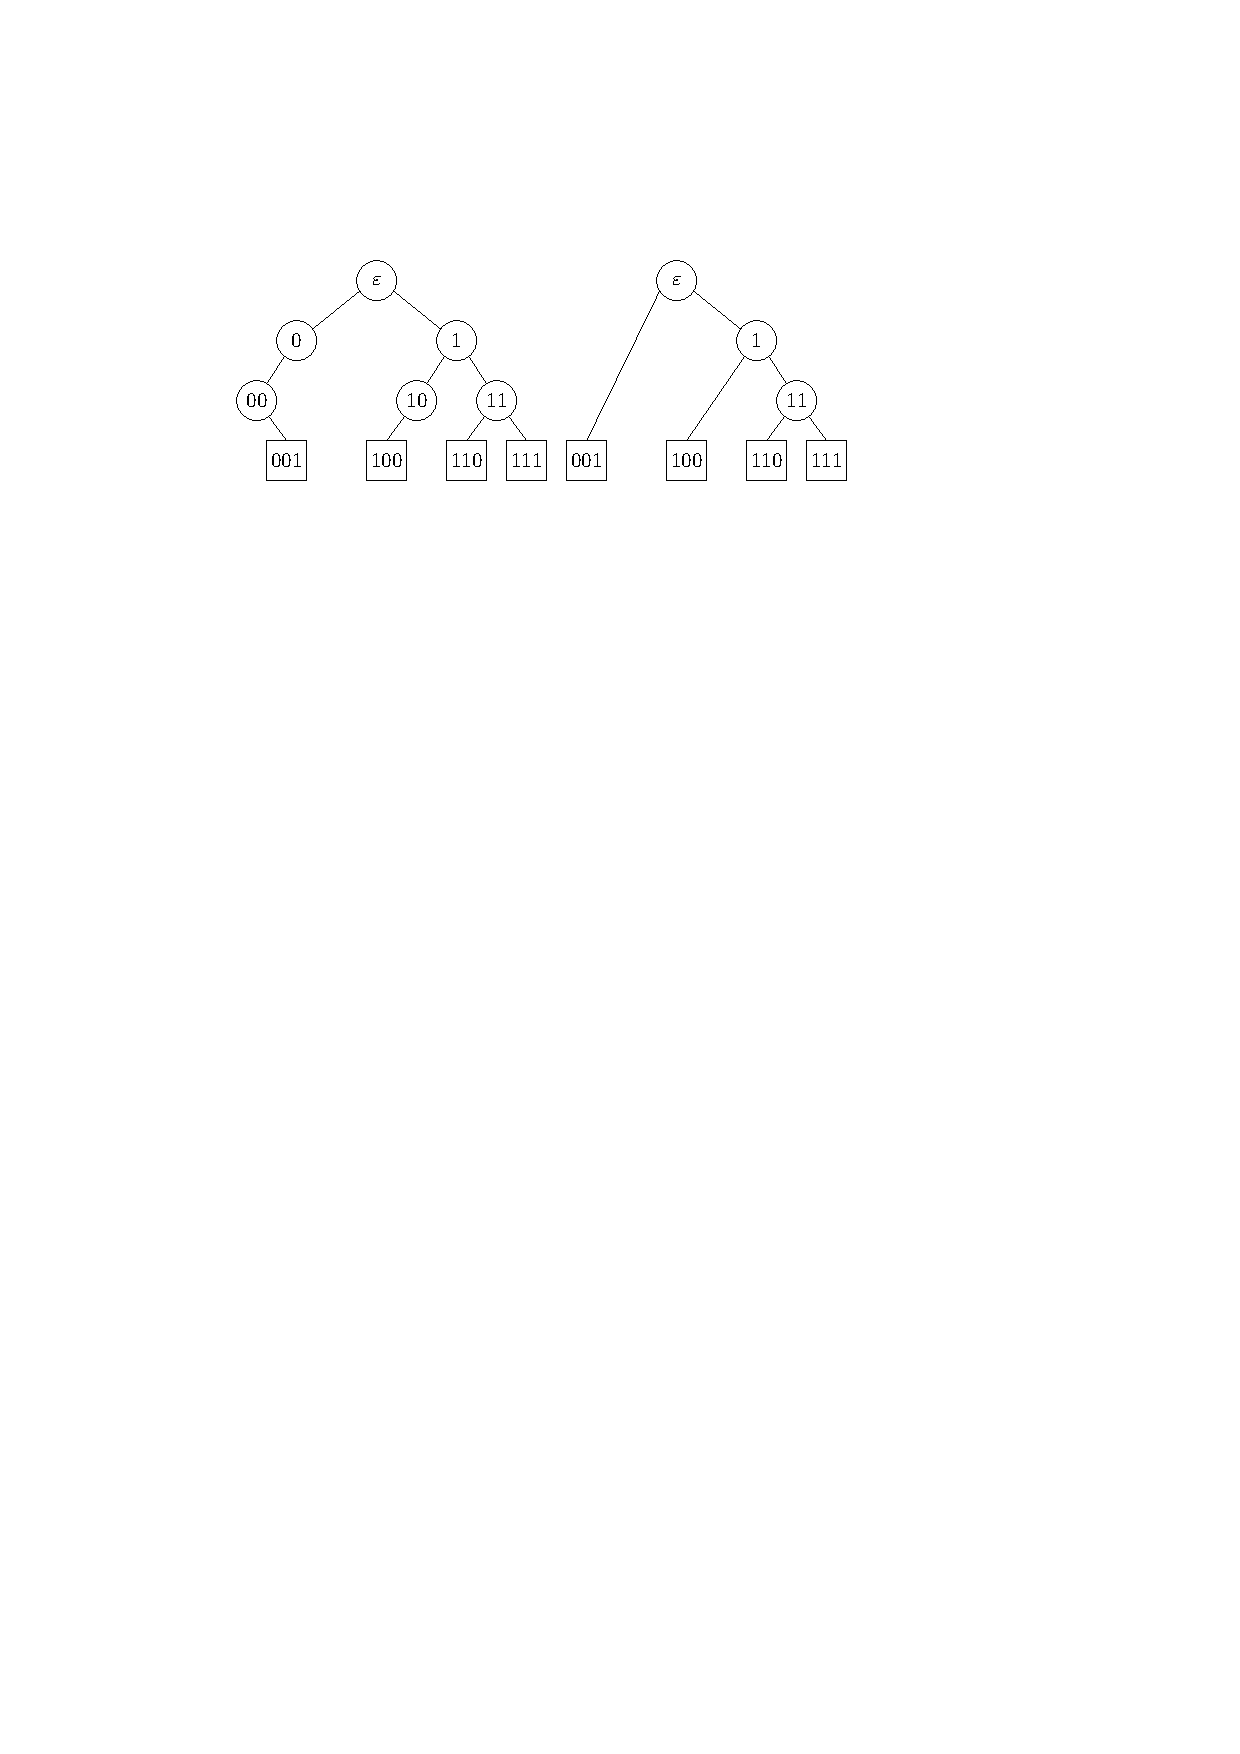
\includegraphics{trie}
  \caption{A trie (left) and a compressed trie (right) for the set 
  000, 100, 110, 111. The nodes are annotated with their
  extents. The longest common prefix of 101 is  10. The 
  lca of 101 in the compressed trie
    is the node labeled 1.}
  \label{fig:trie}
\end{figure}

The \emph{compressed trie} $T$ for $S$ is obtained
from $T'$ by contracting into a single edge each maximal path in $T'$ that
has only nodes with exactly one child.
The root of $T$ corresponds to the highest node of $T'$ that has 
two children.  Every inner node in $T$ has exactly two children,
and $T$ has $n$ leaves. 
Consequently, $T$ has $O(n)$ nodes. 

Let $v$ be a nonroot-node in the compressed trie $T$,
and suppose that $u$ is the parent of $v$ in $T$. Then, 
the extent $e_v$ of $v$ has the form $e_v = e_ubc_v$, 
where $e_u \in \{0, 1\}^*$ is the extent of $u$, $b \in \{0,1\}$ is 
a bit that indicates whether $v$ is the left or the right child
of $u$, and $c_v \in \{0, 1\}^*$ is called the \emph{compressed
path} of $v$. Both $e_u$ and $c_v$ may be empty, but $e_u$
can be empty only if $u$ is the root of $T$. 
We call $n_v = e_ub$ the \emph{name} of $v$.
Next, let $v$ be the root of $T$.
In this case, we set the compressed path $c_v$
to $e_v$, where the extent $e_v$ of the root may
be empty.
Furthermore, we set $n_v = \eps$.

Let $v$ be any node of $T$.
We call the extent $e_v$ 
\emph{internal} if $v$ is an internal node of $T$.
The \emph{skip interval} of $v$ is defined as
$[1, |e_v|]$, if $v$ is the root, and $[|n_v|, |e_v|]$, otherwise.
Given a string $q \in \{0, 1\}^*$ with $|q| \leq w$, the 
\emph{exit node} of $q$, denoted as $\exit(q)$, is the unique node
$v$ in $T$ such that $n_v$ is a prefix of $q$ and either
$e_v = q$ or $e_v$ is not a prefix of $q$.
Figure~\ref{fig:ztrie} illustrates these definitions.

\begin{figure}[t]
\centering
\includegraphics[scale=.80]{zpred-1}
\caption{(above) A compressed trie, the 
related names, and the function $T$ of the associated 
z-fast trie. The skip interval for $v$ is $[7, 14]$. 
Dashed lines show the end of the handles of internal nodes.}
\label{fig:ztrie}
\end{figure}

\subsection{Z-fast Tries and Fat Binary Search}

We recall some key definitions from~\cite{BelazzouguiBoPaVi09}:

\begin{definition}[2-fattest numbers and handles] 
\label{def:twofattest}
Let $a, b \in \N$, $a \leq b$. The \emph{2-fattest number} 
of the interval $[a, b]$ is the unique integer in $[a, b]$ 
that is divisible by the largest power of two. Equivalently, 
it is the integer with the largest number of trailing zeroes 
in its binary representation. The \emph{handle} $h_v$ of a 
node $v$ in a compressed trie is the prefix of $e_v$ whose 
length is the 2-fattest number of the skip interval of $v$
(see Figure~\ref{fig:ztrie}). If the skip interval of $v$ 
is empty (which can happen only at the root), we set 
$h_v = \eps$.
\end{definition}

We remark that if $c$ is the 2-fattest number of $[a, b]$, then 
$c$ is also the 2-fattest number in every subinterval of $[a, b]$ 
that contains it.

\begin{definition}[z-fast trie]
Suppose we are given a set $S \subseteq \{0, 1\}^w$. Let $T$ be the 
compressed trie for $S$. The \emph{z-fast trie on $S$} is 
a function $Z : \{0, 1\}^* \rightarrow \{0, 1\}^*$ such that 
$Z(h_v) = e_v$, for every internal node $v$ of $T$, and such
that any other string is mapped to an arbitrary internal extent
of $T$.\footnote{Recall that the inputs and outputs of $Z$
are represented as two $w$-bit words, encoding the length
and the padded string.}
\end{definition}

Given a z-fast trie $Z$ for $S$, we can determine very 
quickly the name of the exit node for any query string $q \in \{0,1\}^+$.
For this, we use a variant of binary search, called 
\emph{fat binary search}.
The goal is to find the length $|e|$ of the 
longest internal extent $e$ that is a proper 
prefix of $q$. Once $|e|$ is known, the name 
of $\exit(q)$ is obtained as $q\big[0, |e|\big]$.
The fat binary search is started with an initial
search interval $[a,b]$ that is guaranteed
to contain $|e|$. The main difference to
a standard binary search is that we do
not split the search interval on its
midpoint, but on its 2-fattest number.
Furthermore, we maintain the invariant
that the left endpoint of the search interval $a$ 
is the length of an internal extent
of $T$.  This makes the search order more
predictable: all the decision points of the
fat binary search are contained in the z-fast trie
and are readily available after preprocessing.
See the pseudo-code in Algorithm~\ref{algo:query} for details. 
The algorithm reported here, an extension of the 
result from~\cite{BelazzouguiBoVi10}, has two main features:
it imposes very weak requirements on $Z$, and it allows us to start 
the search on a small interval that is subject to
mild conditions. This latter feature will be crucial 
for our main results. The next lemma formally states
the invariant of the fat binary search.

\begin{algorithm}
\KwIn{a string $q \in \{0,1\}^+$, an initial 
search interval $[a,b]$ so that  $a \in [0, |q|]$
and $a = 0$ or $q[0, a - 1]$ is an internal extent of $T$, and
so that $b \in [a, |q|]$ and $b$ is larger than the length 
of the longest internal extent of $T$ that is a proper prefix of $q$}
\KwOut{the name of $\exit(q)$}
\While{$b - a > 1$}{%
$c \gets $ the 2-fattest number in $[a + 1, b - 1]$%
\label{line:2fattest}\;
$e \gets Z(q[0, c - 1])$%
\label{line:qprefix}
\;
\If{$c \leq |e| \wedge e \prec q$
\label{line:prefixtest}
}{%
  \tcp{Move from $[a, b]$ to $[|e|,b]$}
 $a\gets |e|$\;
\label{alg1:reass1} 
} \Else{%
\tcp{Move from $[a, b]$ to $[a, c]$}
$b \gets c$\;
\label{alg1:reass2} 
}
}
\If{$a = 0 \wedge e_\text{root}\neq\eps$}{% 
  \Return $\eps$\;
} \Else{%
  \Return $q[0, a]$\;
}
\caption{Fat binary search in order to 
  determine the name of $\exit(q)$.}
\label{algo:query}
\end{algorithm}

\begin{lemma}\label{lem:correctness}
Let $q \in \{0, 1\}^+$ be a query string.
Let $e_0 = \eps$ and $e_1, e_2, \dots, e_t$ be the internal 
extents of $T$ that are \emph{proper} prefixes of $q$, ordered by 
increasing length.  Let $[a, b]$ be the search interval maintained by 
Algorithm~\ref{algo:query}. Before and after each iteration, the 
following invariants are satisfied: 
\begin{enumerate}
    \item\label{enu:lema} $a = |e_j|$, for some $j$;
    \item\label{enu:lemb} $b > |e_t|$.
\end{enumerate}
It follows that when the algorithm terminates, we have, $a = |e_t|$.
\end{lemma}

\begin{proof}
Consider invariant (\ref{enu:lema}).
At the beginning, the invariant holds
by our assumption on the initial search interval. 
Moreover, the invariant is maintained throughout
the algorithm. Indeed, the value of
$a$ changes only in line~\ref{alg1:reass1} of Algorithm~\ref{algo:query}. 
Suppose that currently we have $a = |e_j|$, for some $j$, and
that line~\ref{alg1:reass1} is executed. Then, we know that $e$ is an 
internal extent, that $|e_j| = a  < c  \leq |e|$, 
and that $e \prec q$. Thus, it follows that $e = e_k$, 
for some $k > j$.

Next, consider invariant (\ref{enu:lemb}).
At the beginning, the invariant holds 
by our assumption on the initial search interval.
To show that the invariant is preserved,
note that $b$ changes only in 
line~\ref{alg1:reass2}.
By invariant (\ref{enu:lema}), at the beginning of
an iteration of the \textbf{while}-loop, we have $a = |e_j|$, 
for some $j$.  
Let $v_{j+1}, \dots, v_{t}$ be the inner nodes in $T$ 
with $e_{v_k} = e_k$, for $k = j + 1, \dots, t$.
Then, the skip intervals of $v_{j+1}, \dots, v_t$ are 
pairwise disjoint, and their union is $[a + 1, |e_t|]$.
Thus, if $c \leq |e_t|$, then $c$ lies in the
skip interval of some $v_k$.
Since $c$ is 2-fattest in $[a + 1, b - 1]$, 
it is also 2-fattest in the skip interval of $v_k$. 
Hence, we have $q[0, c - 1] = h_{v_k}$ and 
$Z(q[0, c - 1]) = e_k$, 
which satisfies $c \leq |e_k|$ and $e_k  \prec q$. 
Thus, line~\ref{alg1:reass2} is executed only if $c > |e_t|$.
The invariant $b > |e_t|$ is preserved.
\end{proof}

We can now show that our fat binary search is correct.
\begin{theorem}
\label{thm:correctnessfbs}
Algorithm~\ref{algo:query} takes at most $\lceil\log(b-a)\rceil$
iterations
and finds the name of $\exit(q)$.
\end{theorem}

\begin{proof}
We first bound the number of iterations. Consider
an interval $[\ell, r]$ and suppose that
$[\ell, r]$ contains at most one multiple
of $2^i$. Furthermore, let $c$ be the 
$2$-fattest number in $[\ell, r]$.
Then, the two subintervals $[\ell, c - 1]$ and 
$[c + 1, r]$ each contain at most one multiple 
of $2^{i-1}$. Indeed, if one subinterval 
contained two such multiples, it would also 
contain a multiple of $2^i$ in its interior. 
However, this multiple would have to be $c$, 
since $[\ell, r]$ contains no other multiple 
of $2^i$, a contradiction. It now follows 
by induction that after splitting the 
interval $[\ell, r]$ at most $i$ times, the 
resulting interval has length at most one. 
Now, since an interval of length $k$ contains at most one multiple of 
$2^{\lceil\log k\rceil}$, the algorithm
has at most $\lceil\log(b-a)\rceil$ iterations.

It remains to argue correctness. 
By Lemma~\ref{lem:correctness}, we know
that if the algorithm terminates, then
$a = |e|$, where $e$ is the longest internal
extent of $T$ that is a proper prefix of $q$,
or $a = 0$, if no such internal extent exists. If $a > 0$ 
then $q[0, a]$ is the name of $\exit(q)$.
If $a = 0$, there may be two 
reasons for this: (a) there is no internal
extent that is a proper prefix of $q$. In this case,
the extent of the root must be non-empty, and
$\exit(q)$ is the root; or (b) the longest internal
extent that is a proper prefix of $q$ is $\eps$.
In this case, this extent is located at the root, and 
$\exit(q)$ is the child of the root
that corresponds to the first bit
of $q$.
All these cases are handled by the
final case distinction in Algorithm~\ref{algo:query}.
\end{proof}

We comment on some implementation aspects of 
Algorithm~\ref{algo:query}.
First, in line~\ref{line:2fattest}, the 2-fattest
number in the interval $[\ell, r]$ with $\ell \leq r$
can be found in constant time with the expression 
\[
(1^w \texttt{ shl } 
\texttt{msb}((\ell - 1) \texttt{ xor } r)) \texttt{ and } r,
\]
where $1^w$ represents the $w$-bit word in which all bits
are set to $1$. Indeed, the 2-fattest number in $[\ell,r]$
is the number n $[\ell, r]$ with the maximum number of trailing zeroes
in its binary representation. To find this number, we identify
the index of the highest valued bit that changes from $0$ to
$1$ when counting from $\ell - 1$ to $r$, (this is
given by $\texttt{msb}((\ell - 1) \texttt{ xor } r))$), and 
we use an appropriate mask to find the corresponding
prefix of $r$. \wolfgang{Make a picture.}
Second, in line~\ref{line:qprefix}, the substring $q[0, c-1]$ 
can also be found in constant
time, using bit shifting to create an appropriate bit mask.
The same holds for the prefix test $e \prec q$ in line~\ref{line:prefixtest}.


\subsection{Implementing the Function $Z$}

We now explain the implementation details of the
z-fast trie $Z$. We split the computation of $Z$ into
two basic components:
\begin{enumerate}
  \item the \emph{handle resolver} $g: \{0,1\}^* \rightarrow \N$ 
    maps each handle $h_v$ of $T$ to the length of the name 
    $n_v$ of its associated 
    node $v$. That is, $g(h_v) = |n_v|$, for every internal node $v$ 
    of $T$. The value $g(h)$ is arbitrary of $h$ is not a handle of $T$;
  \item the \emph{range locator} receives a string $n \in \{0, 1\}^*$.
  If $n = n_v$  is the name of a node $v$ of $T$, it returns the minimum and
  maximum element of $S$ stored in the subtree of $T$
  rooted at $v$, i.e., the smallest element $s_{\lrange(v)}$ and the 
  largest element $s_{\rrange(v)}$ of $S$ that
  have $n_v$ as a prefix. If $n$ is not a valid name in $T$, the range
  locator returns two arbitrary elements $s_\ell$ and $s_r$ from $S$.
\end{enumerate}

These two data structures let us implement several efficient operations
on $T$. In particular, as was also observed by 
\Patrascu~\cite{Patrascu10}, the additional indirection
given by the handle resolver will lead to a space efficient implementation
of the z-fast trie $Z$.
Let $n_v \in \{0, 1\}^*$ be the name of a node $v \in T$. We 
write $\extent(n_v)$ for the extent $e_v$ of $v$. With the range locator,
we can implement the function $\extent(\cdot)$ with constant overhead.

\begin{lemma}\label{lem:getextent}
Suppose that a range locator for $T$ is available. 
Then, the following operation can be implemented
with one call to the range locator and $O(1)$
additional steps.
Given a string $n \in \{0, 1\}^*$: 
if $n$ is the name for a node in $T$, return
$\extent(n)$; if $n$ is not a valid name
in $T$, return an arbitrary valid extent in $T$.
\end{lemma}

\begin{proof}
Given $n$, we use the range locator to find 
two elements $s_\ell$ and $s_r$ in $S$.
If $s_\ell = s_r$, we return $s_\ell$.
Otherwise, we return the longest common prefix of 
$s_\ell$ and $s_r$. This can be done in
$O(1)$ steps, using the \texttt{msb}-operation
and appropriate bit-manipulation.
The procedure certainly returns a valid extent
in $T$, and if $n$ is the actual name of node
$v$ in $T$, then the result is $\extent(n)$, 
as desired.
\end{proof}

Combining Lemma~\ref{lem:getextent} with a handle resolver,
we can implement the z-fast trie efficiently.

\begin{lemma}\label{lem:implementz}
Suppose that a handle resolver and a range locator for $T$ are 
available. Then, 
we can implement the following operation with one call to the
handle resolver, one call to the range locator, and $O(1)$
additional operations:
for any given given string $h \in \{0, 1\}^*$,
if $h$ is a handle for a node in $T$, compute
$Z(h) = \extent(h)$; 
if $h$ is not a valid handle in $T$, return
any valid extent in $T$.
\end{lemma}

\begin{proof}
We use the handle resolver to find the presumptive length
$a$ of the name corresponding to $h$.
We set $n = h[0, a - 1]$,  
and  we use Lemma~\ref{lem:getextent}
to obtain an extent for $n$.
If $h$ is a valid handle, we obtain the required information by
Lemma~\ref{lem:getextent} and by the correctness of the handle 
resolver. If $h$ is not a valid handle, 
Lemma~\ref{lem:getextent} still yields a valid extent in $T$.
\end{proof}

Now, by Theorem~\ref{thm:succinct_retrieval_only_hashtable},
we can implement a handle resolver with constant 
query time, and with $O(n \log w)$ bits of 
space.  Furthermore, if $S = \langle s_1, s_2, \dots, s_n\rangle$ 
is given in lexicographic sorted order and can be accessed in
constant time \wolfgang{What does this mean? Random access to 
a table storing $S$?},
there is a constant-time range locator for $S$ using $O(n\log w)$
bits~\cite{BelazzouguiBoPaVi09}.
\wolfgang{Specific theorem? Put into intro}
This leads to the following theorem.

\begin{theorem}
\label{th:zfast}
Let $S \subseteq \{0, 1\}^w$.
If $S$ is given in lexicographic order and if constant time
access to $S$ is available, the z-fast trie $Z$ for $S$ can be
implemented in $O(1)$ with additional $O(n\log w)$ bits of space.
\qed
\end{theorem}

\subsection{From Exit Nodes to Predecessors}

Now consider a query string $q \in \{0, 1\}^w$.
By our discussion so far, we know that
with fat binary search, we can quickly find the 
(length of) the name of the exit node of $q$, $\exit(q)$. 
Now, we explain how we can use this
information to find $q^-$, the predecessor of $q$ in $S$.
Given $q$ and the length $t$ of the name of $\exit(q)$, 
we denote by  $\pred(q, t)$ the index of $q^-$
in the sorted array $S$.

\begin{lemma}
Suppose that a range locator for $T$ is available.
Let $q \in \{0, 1\}^w$ be a query string and
$t$ the length of the name of $\exit(q)$.
Then, we can compute $\pred(q, t)$ with one 
call to the range locator and with $O(1)$ additional
steps.
\end{lemma}
\begin{proof}
Since the name of $\exit(q)$ is given by $q[0, t - 1]$,
we can use Lemma~\ref{lem:getextent} to compute
the extent $\extent(q[0, t - 1])$ of $\exit(q)$.
This needs one call to the range locator and $O(1)$ 
additional steps.
Then, we check if $q \preceq \extent(q[0, t - 1])$ or 
if the first bit of 
$q$ at which $q$ and $\extent(q[0, t-1])$ differ is a $0$. 
This can be done in constant time, using the \texttt{msb}-function
and appropriate bit-shifting operations..
If so, the index of $q^-$ is $\lrange(\exit(q))-1$.
Otherwise, the index of $q^-$ is 
    $\rrange(\exit(q))$.
\end{proof}

We denote with $\fbs^-(q,a,b)$ the predecessor index computed by 
running Algorithm~\ref{algo:query} (with inputs $q$, $a$, and $b$) 
to obtain the name of $\exit(q)$ and then invoking $\pred(q, t)$.
We remark that the definition above implies that 
by evaluating $\fbs^-(q,0,|q|)$, we can find
the predecessor $q^-$ of a given query string $q$ 
in $O(\log w)$ time, using 
$O(n\log w)$ bits in addition to the sorted array $S$.

\subsection{Using the Range Locator to Check Prefixes}

Let $P \subseteq \Pref(S)$ be a set of prefixes of $S$, and
assume that we have a function $f : P \rightarrow \N$ that 
returns for each $p \in P$ the length of the name of 
$\exit(p)$.
Given a candidate prefix $p \in \{0, 1\}^*$, we would like 
to distinguish whether $p$ belongs 
to $P$ or is not a prefix of any string in $S$.\footnote{Note
that we make no claim for the case that $p$ belongs to
$\Pref(S) \setminus P$.}
Our key observation is that a range locator, combined with access 
to the sorted array $S$, can be used to extend 
$f$ so that it returns a special value $\bot$ outside of $\Pref(S)$:

\begin{theorem}
\label{th:pref}
Let $P \subseteq\Pref(S)$, and let $f: P \rightarrow \N$ be 
given by $f(p) = |n_{\exit(p)}|$, for $p \in P$.
Suppose that $f$ can be computed in constant time,
and that we have access to the sorted
array $S$ and to a range-locator for $S$ that
requires constant time.
Then, we can extend 
$f$ to a constant-time function $\widehat{f}: \{0, 1\}^* \rightarrow \N
\cup \{ \bot \}$ such that $\widehat{f}(p)=|n_{\exit(p)}|$, for 
all $p \in P$, and $\widehat{f}(p) = \bot$, for
all $p \not\in\Pref(S)$.
\end{theorem}

\begin{proof}
Given $p \in \{0, 1\}^*$, we invoke
$f$ to compute a candidate length $t = f(p)$ 
for $n_{\exit(p)}$.
If $t > |p|$, we return $\bot$.
Otherwise,  we use the presumptive
name $p[0, t - 1]$ of $\exit(p)$ 
in Lemma~\ref{lem:getextent} to compute 
the extent $e$ of $\exit(p)$. Now, 
if $p  \preceq e$, we return $f(p)$, otherwise we return $\bot$.

If $p\in P$, then $f(p) = |n_{\exit(p)}| \leq |p|$, and we
compute correctly the extent of $\exit(p)$, so we return 
$f(p)=|n_{\exit(p)}|$.
If $p \not\in \Pref(S)$, then the test if 
$p \preceq e$ must fail for every extent in $T$. 
Hence, in this case, last step returns $\bot$.\footnote{Observe 
that actually $\widehat f$ will return the length 
of the name of the exit node for all prefixes in a set $\hat P$ that 
satisfies $P\subseteq \hat P\subseteq\Pref(S)$.}
\end{proof}

\section{Static Locally Sensitive Predecessor Search}
\label{sec:pred}

We combine Theorems~\ref{th:zfast} and~\ref{th:pref} 
to answer predecessor queries in a time that depends 
on the distance between the query string $q$ and its 
predecessor and successor in $S$. The idea 
is to store selected prefixes from $\Pref(S)$
to reduce significantly the initial search interval of
Algorithm~\ref{algo:query} (by increasing the parameter $a$).
We devise two distinct predecessor algorithms whose 
performance depends on the short and on the
long distance between the $q$ and $S$:
both algorithms use the setup from Theorem~\ref{th:pref}, but with 
different choices of the function $f:P\to \N$. 

\subsection{Short-distance predecessor algorithm}
\label{sec:short-distance}

We use techniques inspired by the work of Bose 
et al.~\cite{BoseDoDuHoMo13} to obtain a
query time that depends on the short distance $d(q, S)$ 
between the query $q$ and $S$. For this, we
consider a sparse set $P$ of prefixes from which
we can start the fat binary search.
It is defined as follows:
\[
	P=\bigl\{\,s\bigl[0,w-2^{2^i} - 1\bigr] \mid s \in  S \text{ and }
	i=0,\dots,\lfloor\log(\log w - 1)\rfloor\,\bigr\}.
\]
To store the function $f: P\to \N$ used in Theorem~\ref{th:pref}, 
we define a subset of $P$:
\[
Q=\bigcup_{\text{node $v$ of $T$}}
\min{}_\preceq\{\,p\in P\mid n_v \preceq p\preceq e_v\,\}
\]
For every node $v$ of $T$, the set $Q$ contains
the shortest string in $P$ that sits between the name and the extent
of $v$ (if any). 
By Theorem~\ref{thm:succinct_retrieval_only_hashtable},
we can store a dictionary that maps every element 
$q \in Q$ to $|n_{\exit(q)}|$ in space $O(n \log w)$ as $|Q|\leq n$.
Furthermore, by Theorem~\ref{thm:bloomier_filter},
we can store another dictionary that maps
every $p\in P$ to the smallest index $i$ such that 
$p[0,w-2^{2^i} - 1]\in Q$.
Since $|P| = O(n \log\log w)$,
this map takes $O(n\log\log w\log\log\log w) = O(n\log w)$ bits. 
To compute $f(p)$, we first find the index $i$ for $p$ in 
the second map, and then we query the first map with 
$p\bigl[0, w - 2^{2^i} -1\bigr]$. 

Now, our strategy is to 
evaluate the function $f$ 
with prefixes of the query string $q$ 
of decreasing lengths.
More precisely, at iteration $i$, we evaluate
$f(p)$ with the prefix $p$ of $q$ with 
length $t = w-2^{2^i}$. 
If this succeeds, we have found a valid prefix of $q$ in $T$,
and we can proceed with the fat binary search.
If not, we evaluate for 
$f(p+1)$ and for $f(p-1)$. If this succeeds, it is
easy to find $q^-$ with the range locator.
If none of our tests succeeds, we proceed to the next
iteration $i+1$. See Algorithm~\ref{algo:pred-short} 
for the details.
\begin{algorithm}
\KwIn{a query string $q\in \{0, 1\}^w$}
\KwOut{the index $j$ such that $S[j] = q^-$}
 $i \gets 0$\;
\While{$2^{2^i} \leq w/2$}{%
  $p \gets q\bigl[0, w-2^{2^i} - 1\bigr]$\;
  $t \leftarrow \widehat{f}(p)$\;
  \If{$t \neq \bot$ }{%
       $e \gets \extent(q[0,t-1])$\;
       \If{$e\prec q$}{%
           \tcp{We found a long extent}
           \Return{$\fbs^-(q,|e|,w)$}\;
	   \label{line:ret1}
       } \Else {
       \tcp{We exit at the node of name $q[0, t-1]$}
       \Return{$\pred(q,t)$} 
       \label{line:ret2}
       }
  }
  $t \gets \widehat{f}(p+1)$\;
  \If{$t \neq \bot$}{%
    \tcp{$q^-$ is the predecessor of $p+1$} 
    \Return $\lrange((p+1)[0,t-1])-1$ 
    \label{line:ret3}
  }
  $t \leftarrow \widehat{f}(p-1)$\;
  \If{$t \neq \bot$}{%
    \tcp{$q^-$ is the successor of $p-1$} 
    \Return $\rrange((p-1)[0,t-1])$  
  }
  $i \gets i + 1$
}
\tcp{Standard search (we found no prefix long enough)}
\Return{$\fbs^-(q,0,w)$}
\caption{Short-distance speedup.}
\label{algo:pred-short}
\end{algorithm}

The following lemma helps us bound the number of
iterations of Algorithm~\ref{algo:pred-short}.
\begin{lemma}
\label{lemma:hitpref}
Let $q \in \{0, 1\}^w$ be a query string.
Let $j \in \N$ with $j \leq w-\log d(q,S)$ be given, 
and set $p=q[0,j - 1]$. 
Then, at least one of $p$, $p+1$, or $p-1$ 
belongs to $\Pref(S)$. 
\end{lemma}

\begin{proof}
There are $2^{w-j}$ strings in $\{0, 1\}^w$
with prefix $p$ ($q$ being one of them), and the same holds
for $p - 1$ and $p + 1$. 
Let $s$ be the string in $S$ that realizes
$d(q, S)$, i.e., $s = q^-$ or $ s = q^+$.
Then, by our assumption on $j$, we have $|q-s| \leq 2^{w-j}$, 
so $s$ must have prefix either $p$ or $p + 1$ or $p-1$.
\end{proof}


\begin{theorem}
Algorithm~\ref{algo:pred-short} returns the predecessor of $q$
in time $O(\log\log d(q,S))$, using an index with 
$O(n \log w)$ bits of space (in addition to the space 
to store the elements of $S$).
\end{theorem}

\begin{proof}
First, we show correctness. If we reach the first return
instruction in Line~\ref{line:ret1}, then $e$ is a valid 
extent and a prefix of $q$, so we start correctly a
fat binary search. At the second return instruction
in Line~\ref{line:ret2}, we know the $q[0, t - 1]$ is
the name of a node $v$, but the extent of 
$v$ is not a prefix of $q$, so
$q$ exits exactly at $v$, and again we return the correct answer. 
If $p + 1$ is a valid prefix of some element of $S$, but $p$ is not, 
then the predecessor
of $p$ is the predecessor of the least element prefixed by $p + 1$, which we
return in Line~\ref{line:ret3} (and analogously for $p - 1$).

Next, we argue about the running time.
By Lemma~\ref{lemma:hitpref}, we will hit a prefix in our set $P$ as soon as
$w - 2^{2^i} \leq w - \log d(q,S)$, that is, as soon as 
$i > \log\log\log d(q, S)$. If $i$ is the
smallest integer satisfying the latter condition, then 
$i - 1 \leq \log\log\log d(q, S)$, so $2^{2^i} \leq (\log d(q, S))^2$, 
which guarantees that the fat binary
search, which starts from an extent of length at least $|e| \geq t \geq
w - 2^{2^i} \geq w - (\log d(q, S))^2$, will complete in time 
$O(\log b - a)=O(\log\log d(q, S))$ (see Theorem~\ref{thm:correctnessfbs}). 
If we exit from the loop,
it means that $i > \log\log\log d(q, S)$ which implies $2^{2^i}>w/2$, hence
$(\log d(q,S))^2>w/2$, so the last fat binary search  taking $O(\log w)$
steps to complete) is still within our time bounds.
\end{proof}

\subsection{Long-distance predecessor algorithm}
\label{sec:long}

We now discuss Algorithm~\ref{algo:pred-long}, whose 
running time depends on long
distances. Let $P$ be the set obtained by ``cutting''
every internal extent $e_v$ to the length of the smallest power of 
$2$ (if any) in the skip interval of $v$, that is:
\[
P =\bigcup_\text{$v$ internal}\{\,e_v[0,2^k -1] \mid 2^k \in
	[|n_v|, |e_v] \text{ and $k$ is the smallest possible}\,\}.
\]
where $v$ ranges over all nodes. This time, we
have at most one prefix per node, so $|P| = O(n)$, and 
the function $f$ required by Theorem~\ref{th:pref} can be stored 
in $O(n\log w)$ bits, by Theorem~\ref{thm:succinct_retrieval_only_hashtable}. 

Algorithm~\ref{algo:pred-long} keeps track of the length $a$ of an
internal extent that is known to be a prefix of $q$. At each step, we 
try to find another extent by probing a prefix of $q$ whose 
length is the smallest power of $2$ larger than
$a$. By the construction of $P$, we can miss the longest
prefix length at most by a factor of two. 

\begin{lemma}
\label{lemma:shortinprefs}
Let $q \in \{0, 1\}^w$ be a query string,
and let $p \in \Pref(S)$ with 
$|p| > w - \log D(q,S)$ and
$p \preceq q$. Then, 
the elements in $S$ with prefix $p$
are either all at most as large or all
at least as large as $q$.
\end{lemma}

\begin{proof}
Since $|p| > w - \log D(q, S)$, we have
that $p$ is a prefix of less than
$2^{\log D(q,S)} = D(q, S)$ strings.
From the definition of $D(q, S)$ it follows
that $|q^+ - q^-| \geq D(q, S)$, so $p$
cannot be a prefix of both $q^+$ and $q^-$.
Now, since the set of strings in $S$ 
with prefix $p$ forms an interval, all elements
in $S$ with prefix $q$ are either all at most as large
or all at least as large as $q$.
\end{proof}


\begin{theorem}	
\label{thm:pred-long}
Algorithm~\ref{algo:pred-long} returns the predecessor of  $q$
in time $O(\log(w-\log D(q, S)))$, using an index with 
$O(n \log w)$ bits of space (in addition to the space 
to store the elements of $S$).
\end{theorem}

\begin{proof}
First, we show correctness. An easy induction shows that throughout
the algorithm, $a$ is either $0$ or the length of an 
internal extent that is a prefix of $q$. 
Then, it follows that since $[a + 1,w - 1]$ is a union of 
consecutive skip intervals and since
the smallest power of $2$ in interval $[a + 1,w - 1]$ is
a fortiori the smallest power of two in a skip interval of $T$,
that of $q[0, m-1]$ is in $\Pref(S)$, then $q[0, m-1]$ must be in $P$.
Thus, if $t = \bot$, Theorem~\ref{th:pref} implies that $m$
must be larger than the length of the longest internal extent
that is a proper prefix of $q$, 
so if we exit at the first return
instruction in Line~\ref{line:retb1}, 
the fat binary search completes correctly. On the other hand, 
if $t \neq \bot$,
we know that $q[0,t - 1]$ is the name of a node $v$ in $T$.
If  
$q$ is smaller than the smallest leaf
under $v$ (or larger than the largest such under $v$),
we immediately know the
predecessor and can safely return with a correct value
in line~\ref{line:retb2} or~\ref{line:retb3}. The return instruction
after the loop in line~\ref{line:retb4} is trivially correct.

Next, we discuss the running time. Observe that when $m > w - \log D(q, S)$,
then either the string $q[0,m -1]$ will not be in 
$\Pref(S)$ (by Lemma~\ref{lemma:shortinprefs}) and thus 
$t=\bot$, or $q$ will be larger (or
smaller) than every element of $S$ prefixed by $q[0,t-1]$, 
which will cause a loop exit at one of the last two \textbf{if}-instructions. 
Since $m$ gets at
least doubled at each iteration, this will happen 
after at most $\log(w-\log D(q,S))$ iterations; moreover, 
$m \leq 2a$ (because there is always a power of $2$ in the interval 
$[a + 1, 2a]$), so the fat binary search in line~\ref{line:retb1}
will take no more than $\log(m-a)\leq \log a\leq \log (w-\log D(q,S))$ steps.
If the loop exits naturally, then there is a prefix of $q$ belonging to 
$\Pref(S)$ and longer than $w/2$, hence $w-\log D(q, S)\geq w/2$ and 
the fat binary
search at the end of the loop will end within the prescribed time bounds.
\end{proof}

\begin{algorithm}
\KwIn{a query string $q \in \{0, 1\}^w$}
\KwOut{the index $i$ such that $S[i]=q^-$}

 $a \gets 0$\;
\While{$a<w/2$}{%
  $m \gets \text{least power of $2$ in $[a+1,w-1]$}$\;
  $t \gets \widehat f(q[0, m-1])$\;
  \If{$t = \bot$}{%
     \Return{$\fbs^-(q,a,m)$}
     \label{line:retb1}
     \tcp{We obtained the longest possible prefix} 
  }
  $p \gets q[0,t-1]$\;
  \If{$S[\lrange(p)]\geq q$}{%
    \Return{$\lrange(p)-1$}
    \label{line:retb2}
  }
  \If{$S[\rrange(p)]<q$}{%
    \Return $\rrange(p)$
    \label{line:retb3}
  }
  $a \gets |\extent(p)|$ 
  \tcp{This is a valid extent}
}
\Return{$\fbs^-(q, a, w)$}
\label{line:retb4}

\caption{Long-distance speedup.}
\label{algo:pred-long}
\end{algorithm}

Finally, we can combine our improvements for short and long 
distances, obtaining an algorithm that is
efficient when the query $q$ is either very close to or very far 
from $q^-$ or $q^+$:

\begin{corollary}
It is possible to compute the predecessor of a query $q$ in a set $S$
of $n$ elements in time $O(\log \min \{\,\log d(q, S), w - \log D(q,S)\,\})$, 
using an index that
requires $O(n \log w)$ bits of space (in addition to the space
needed to store the elements of $S$).
\end{corollary}

\section{Dynamic Short-Distance Predecessor Search}
\label{sec:dyn_pred}

We will now explain how to make our data
structure
from Section~\ref{sec:short-distance} dynamic.
The basic approach remains the same.
However, in contrast to the static case, we now 
maintain the compressed trie $T$ explicitly. 
This means that we do not assume that $S$
is given in a static read-only array with constant
time access, but that the elements of $S$
are stored in a trie that changes dynamically throughout
the algorithm. In particular, our space bounds must also 
include the bits to represent $S$, so the best 
that we can hope for is a data structure that uses $O(nw)$
bits, where $n$ is the current size of $S$. This less restrictive
space regime simplifies some aspects of the algorithm. For example,
the z-fast trie for $S$ can now be maintained explicitly in a
dynamic dictionary. The greatest challenge now is to maintain
the dynamic trie $T$ under the required time bounds and to provide
a fast way to go from the exit node of a given query string $q$ to the 
predecessor of $q$.

More precisely, the compressed trie $T$ is maintained as
an explicit pointer structure where the nodes are represented
as records with parent and
child pointers between them. The leaves of $T$ are
linked in sorted order. For each node
$v$ of $T$, we store the extent $e_v$,
so given a node $v$ and the pointer structure
of $T$, we can easily derive all the associated
information for $v$ in constant time, i.e., the extent $e_v$, 
the name $n_v$, the compressed path $c_v$, the handle $h_v$, and the skip 
interval for $v$.
Furthermore, we need a structure similar to the range locator 
that is given a node $v$ of $T$ and provides pointers to
the largest and the smallest element of $S$ in the subtree
$T_v$ of $T$ that is rooted at $v$. This structure is more non-trivial
to handle dynamically in the desired time bounds, and we will elaborate
on this below in Section~\ref{sec:rangeloc}. 
Finally, the z-fast trie is stored as an explicit
dynamic dictionary structure as given by 
Theorem~\ref{thm:succinct_retrieval_only_hashtable}.

\subsection{Performing a Random Shift}

Since our dynamic algorithm must be able to update the
compressed trie explicitly, we need to be able to get hold
of the exit node $\exit(q)$ in $T$ for any given element 
$q \in \{0, 1\}^w$. To make sure that this can be done efficiently,
we need that $\exit(q)$ lies at a level of $T$ that corresponds to
the desired running time. Since this
does not necessarily need to be the case, we use a trick of 
Bose~\etal~\cite{BoseDoDuHoMo13}.
The idea is to perform a random shift of the universe to
make sure that the distance between two fixed elements
is reflected by the expected length of their longest common prefix. 

More precisely, during initialization, we pick a random 
string $r \in \{0, 1\}^w$ which is fixed throughout 
the remainder of the algorithm. We
add $r$ to all the elements that appear during a
query or an update. Our data structure works internally
with strings of length $w + 1$, so we interpret
the result as an element of the
\emph{extended universe} $\{0, 1\}^{w + 1}$, possibly
obtained by adding a leading $0$-bit.
The utility of this method is shown in
the following lemma, whose proof we include for completeness:

\begin{lemma}[Lemma 4 in \cite{BoseDoDuHoMo13}]
\label{lemma:delta_lca_loglog_delta}
Let $x, y \in \{0, 1\}^w$ be two distinct fixed strings.
Let $r \in \{0, 1\}^w$ be picked uniformly at random.
Then, the expected length of the longest common
prefix of $x + r$ and $y + r$, interpreted
as strings from $\{0, 1\}^{w+1}$, possibly with 
a leading $0$-bit,
is $w - \Theta(\log|x - y|)$.
\end{lemma}

\begin{proof}
Suppose without loss of generality that $x < y$, 
and write $\Delta = y - x$.
The \emph{height} of a string 
$a \in \{0, 1\}^{w+1} \setminus \{ 1^{w+1}\}$
is the number $h \in \{0, \dots, w\}$ such that $a$ 
ends with $01^{h}$. The \emph{height} of an interval
$[a, b]$ of strings from $\{0, 1\}^{w+1} \setminus \{ 1^{w+1}\}$ 
is the maximum height of any string in the interval
$[a, b]$. Consider the randomly shifted strings
$x + r$ and $y + r$. Then, the length of the 
longest common prefix of $x + r$ and $y + r$ is $w - h$,
where $h$ is the height of the interval $[x + r, y + r - 1]$.
Thus, it suffices to show that the expected height of the
interval $[x + r, y + r - 1]$ is $\Theta(\log \Delta)$.

In $\{0, 1\}^{w+1} \setminus \{ 1^{w+1}\}$, there are
$2^{w - h}$ strings of height $h$, for $h = 0, \dots, w$.
The probability that a fixed string $a$ of height $h$
ends up in the interval $[x - r, y + r - 1]$ is the same
as the probability that $a - r$ ends up in the interval 
$[x, y - 1]$, which is at most $\Delta/2^w$. Thus,
the probability that $[x + r, y + r - 1]$ contains
an element of height $h$ is at most 
$\min \{1, \Delta/2^h\}$, and 
the expected height of the interval 
$[x + r, y + r - 1]$  is at most
\[
\sum_{h = 1}^w  \min \left\{1, \frac{\Delta}{2^h} \right\} \leq 
\sum_{h = 1}^{\lceil \log \Delta \rceil } 1 +  
\sum_{h =  \lceil \log \Delta \rceil  + 1 }^w  \frac{\Delta}{2^h} 
\leq  \lceil \log \Delta \rceil  +  1.
\]
On the other hand, the interval $[010^{w - 1}, 011^{w - 1}]$ and the interval
$[100^{w - 1}, 101^{w - 1}]$ each contain at least $2^{w - 2 - h}$ strings
of height $h$, for $h = 0, \dots, w - 2$. Now, if 
\[
\big\vert [x, y -1] \cap [000^{w - 1}, 001^{w - 1}] \big\vert
\geq \frac{\Delta}{2},
\]
then for a fixed string
$a \in [010^{w - 1}, 001^{w - 1}]$, the probability that $a - r$
ends up in $[x, y - 1]$ is at least $\Delta/2^{w + 1}$, and similarly,
if 
\[
\big\vert [x, y -1] \cap [010^{w - 1}, 011^{w - 1}] \big \vert 
\geq \frac{\Delta}{2},
\]
then for a fixed string
$a \in [100^{w - 1}, 101^{w - 1}]$, the probability that $a - r$
ends up in $[x, y - 1]$ is at least $\Delta/2^{w + 1}$.
In either case,
the probability that $[x + r, y + r - 1]$ contains
an element of height $h$ is at least 
$\min \{1, \Delta/2^{h + 3}\}$, and 
the expected height of the interval 
$[x + r, y + r - 1]$  is at least
\[
\sum_{h = 1}^{w - 2}  \min \left\{1, \frac{\Delta}{2^{h + 3}} \right\} \geq 
\sum_{h = 1}^{\lfloor \log \Delta \rfloor - 3 } 1 +  
\sum_{h =  \lfloor \log \Delta \rfloor  -2 }^{w - 2}  \frac{\Delta}{2^h} 
\geq  \lfloor \log \Delta \rfloor - 3.
\]
Thus, the expected height of the interval $[x + r, y + r - 1]$
is $\Theta(\log \Delta)$, and the claim follows.
\end{proof}

\subsection{Explicit z-Fast Tries and Explicit Fat Binary Search}

Since we have $O(nw)$ bits of storage at our
disposal, and since the trie $T$ is maintained
as an explicit pointer structure, we can now
also use more explicit versions of the z-fast trie
and of the fat binary search.

\begin{definition}[explicit z-fast trie]
Suppose we are given a set $S \subseteq \{0, 1\}^w$, and a fixed
random shift $r \in \{0, 1\}^w$. Let $T$ be the 
compressed trie for $S + r$, represented as a pointer structure. 
The \emph{explicit z-fast trie on $S$} is 
a function $Z' : \{0, 1\}^* \rightarrow V(T)$, where
$V(T)$ denotes the node set of $T$. We require that
$Z'(h_v) = v$, for every internal node $v$ of $T$,
and that any other string is mapped to an arbitrary
inner node of $T$.
\end{definition}

\begin{algorithm}
\KwIn{a string $q \in \{0,1\}^+$, an initial 
search interval $[a, b]$ so that  $a \in [0, |q|]$
and $a = 0$ or $q[0, a - 1]$ is an internal extent of $T$, and
so that $b \in [a, |q|]$ and $b$ is larger than the length 
of the longest internal extent of $T$ that is a proper prefix of $q$}
\KwOut{a pointer to $\exit(q)$}
\While{$b - a > 1$}{%
$c \gets $ the 2-fattest number in $[a + 1, b - 1]$\;
$v \gets Z'(q[0, c - 1])$\;
\If{$c \leq |e_v| \wedge e_v \prec q$}{%
  \tcp{Move from $[a, b]$ to $[|e_v|,b]$}
 $a\gets |e_v|$\;
} \Else{%
\tcp{Move from $[a, b]$ to $[a, c]$}
$b \gets c$\;}
}
\If{$a = 0 \wedge e_\text{root}\neq\eps$}{% 
  \Return the root of $T$\;
} \Else{%
  \Return the child of $v$ corresponding to $q[|e_v|]$\;
}
\caption{Explicit fat binary search in order to 
  determine a pointer to $\exit(q)$.}
\label{algo:query-explicit}
\end{algorithm}

Since there are $O(n)$ nodes in $T$, and since a pointer
to a node in $T$ can be represented with $O(w)$ bits,
an explicit z-fast trie can be implemented with a dynamic
dictionary of $O(nw)$ bits, as described in 
Theorem~\ref{thm:succinct_retrieval_only_hashtable} (since
our trie $T$ is stored explicitly, it is easy to make
sure that $Z'$ returns only valid internal nodes
of $T$). Using
an explicit z-fast trie, we can also modify the fat binary
search to return an explicit pointer
to the exit node of the query string. 
This is shown in Algorithm~\ref{algo:query-explicit}.

Algorithm~\ref{algo:query-explicit} has
the same properties as Algorithm~\ref{algo:query},
and the following theorem is completely analogous to
Theorem~\ref{thm:correctnessfbs}.

\begin{theorem}
\label{thm:correctnessfbs-explicit}
Algorithm~\ref{algo:query-explicit} needs at most $\lceil\log(b-a)\rceil$
iterations
and finds a pointer to $\exit(q)$.
\end{theorem}

\begin{proof}
The argument is identical to the proof of Theorem~\ref{thm:correctnessfbs}.
In particular, the algorithm maintains the invariant from
Lemma~\ref{lem:correctness}, and the running time 
follows as before.
\end{proof}

We will denote an invocation of Algorithm~\ref{algo:query-explicit}
with parameters $q$, $a$, and $b$ as $\fbs_e^{-}(q, a. b)$.

\subsection{Locating the Exit Node for a Query String}

After performing the random shift from 
Lemma~\ref{lemma:delta_lca_loglog_delta}, we can use a simplified 
variant of Algorithm~\ref{algo:pred-short} together with
the explicit fat binary search from Algorithm~\ref{algo:query-explicit}
to find an exit node for a query string $q \in \{0, 1\}^w$.
Our algorithm again uses a sparse set $P$ of prefixes that
serve as starting points for the fat binary search. For a
fixed random shift $r \in \{0, 1\}^w$, it is defined as 
follows:
\[
  P = \bigl\{\, (s + r)\bigl[0,w - 2^{2^i}\bigr] \mid s \in  S \text{ and }
	i = 0,\dots,\lfloor\log(\log w - 1)\rfloor\,\bigr\}.
\]
Our goal is to implement a function 
$g : \{0, 1\}^{w + 1} \rightarrow V(T) \cup \{\perp\}$ such that
for every $p \in P$, we have $g(p) = \exit(p)$, and such 
that $g(p) = \perp$ for all $p \not\in \Pref(S + r)$.
For this, we consider the set 
\[
Q=\bigcup_{\text{node $v$ of $T$}}
\min{}_\preceq\{\,p\in P\mid n_v \preceq p\preceq e_v\,\},
\]
and we maintain two dynamic dictionaries:
one dictionary that maps every $p \in P$ to the smallest
index $i$ such that $p[0, w - 2^{2^i} - 1] \in Q$, and
another dictionary that maps every element $q \in Q$ to
a pointer to the corresponding node in $T$.
Using the dictionary from 
Theorem~\ref{thm:succinct_retrieval_only_hashtable},
the  first dictionary requires 
$O(n \log \log w \log (w - \log (n \log \log w)) 
+  n \log\log w \log\log\log n) = O(nw)$ 
bits, since $|P| = O(n \log\log w)$,
and since each entry has $O(\log w)$ bits.
The second dictionary requires $O(nw)$ bits, since $|Q| = O(n)$ and
since each entry requires $O(w)$ bits.
To evaluate $g(p)$ in constant time, we first query the first dictionary with
$p$, and then the second dictionary table with the
result of the first lookup. Since $T$ is stored
explicitly, we can then check easily whether this results
in the desired node $v$ of $T$. If so, we return $v$, otherwise,
we return $\perp$. Now, the search algorithm is an easy
adaptation of Algorithm~\ref{algo:pred-short}, it is shown
in Algorithm~\ref{algo:pred-short-dynamic}.

\begin{lemma}
\label{lem:delta_fast_expected_lca}
Let $S \subseteq \{0, 1\}^w$ and let $r \in \{0, 1\}$
be a fixed random shift. Let $T$ be 
a compressed trie for $S + r$. 
Let $q \in \{0, 1\}^w$. 
We can find the exit node for $q + r$ in $T$  
in expected time $O(\log\log d(q, S))$.
The expectation is
over the random choice of the shift $r$. 
\end{lemma}

\begin{proof}
Suppose without loss of generality that 
$d(q, S) = |q - q^-|$.
By Lemma~\ref{lemma:delta_lca_loglog_delta},
the expected length of the longest common
prefix of $q + r$ and $q^- + r$ is 
$w - \Theta(\log d(q, S))$.
Thus, since $x \mapsto \log\log\log x$ is a concave function, 
Jensen's inequality shows that we will
hit a prefix in $P$ after an expected number of  $O(\log \log \log d(q, S))$
iterations. After that, 
Theorem~\ref{thm:correctnessfbs-explicit} and
Jensen's inequality show that
the expected time for the fat binary search is 
$O(\log \log \log d(q, S))$.
\end{proof}


\begin{algorithm}
\KwIn{a query string $q\in \{0, 1\}^w$ and a fixed random shift 
$r \in \{0, 1\}^w$}
\KwOut{a pointer to the exit node of $q$ in $T$}
 $i \gets 0$\;
\While{$2^{2^i} \leq (w + 1)/2$}{%
  $p \gets (q + r)\bigl[0, w - 2^{2^i}\bigr]$\;
  $v \leftarrow g(p)$\;
  \If{$v \neq \bot$ }{%
       \If{$e_v \prec q + r$}{%
           \tcp{We found a long extent}
           \Return{$\fbs_e^-(q + r,|e_v|,w + 1)$}\;
       } \Else {
       \tcp{$v$ is the desired exit node}
       \Return{$v$} 
       }
  }
  $i \gets i + 1$
}
\tcp{Standard search (we found no prefix long enough)}
\Return{$\fbs_e^-(q,0, w + 1)$}
\caption{Short-distance speedup in the dynamic setting.}
\label{algo:pred-short-dynamic}
\end{algorithm}

\subsection{Finding the Predecessor Node}
\label{sec:rangeloc}

Algorithm~\ref{algo:pred-short-dynamic}
finds the exit node for a given query string
$q \in \{0, 1\}^w$. However, we still need
a structure to go from $\exit(q)$ to the
node that stores the predecessor of $q$ in $S$.
More precisely, we need to maintain for each node $v \in T$ the
leftmost and the rightmost element in the subtree $T_v$ of $T$
that is rooted in $T$.
This information needs to be updated quickly as 
$S$ changes dynamically.

\begin{figure}
\centering
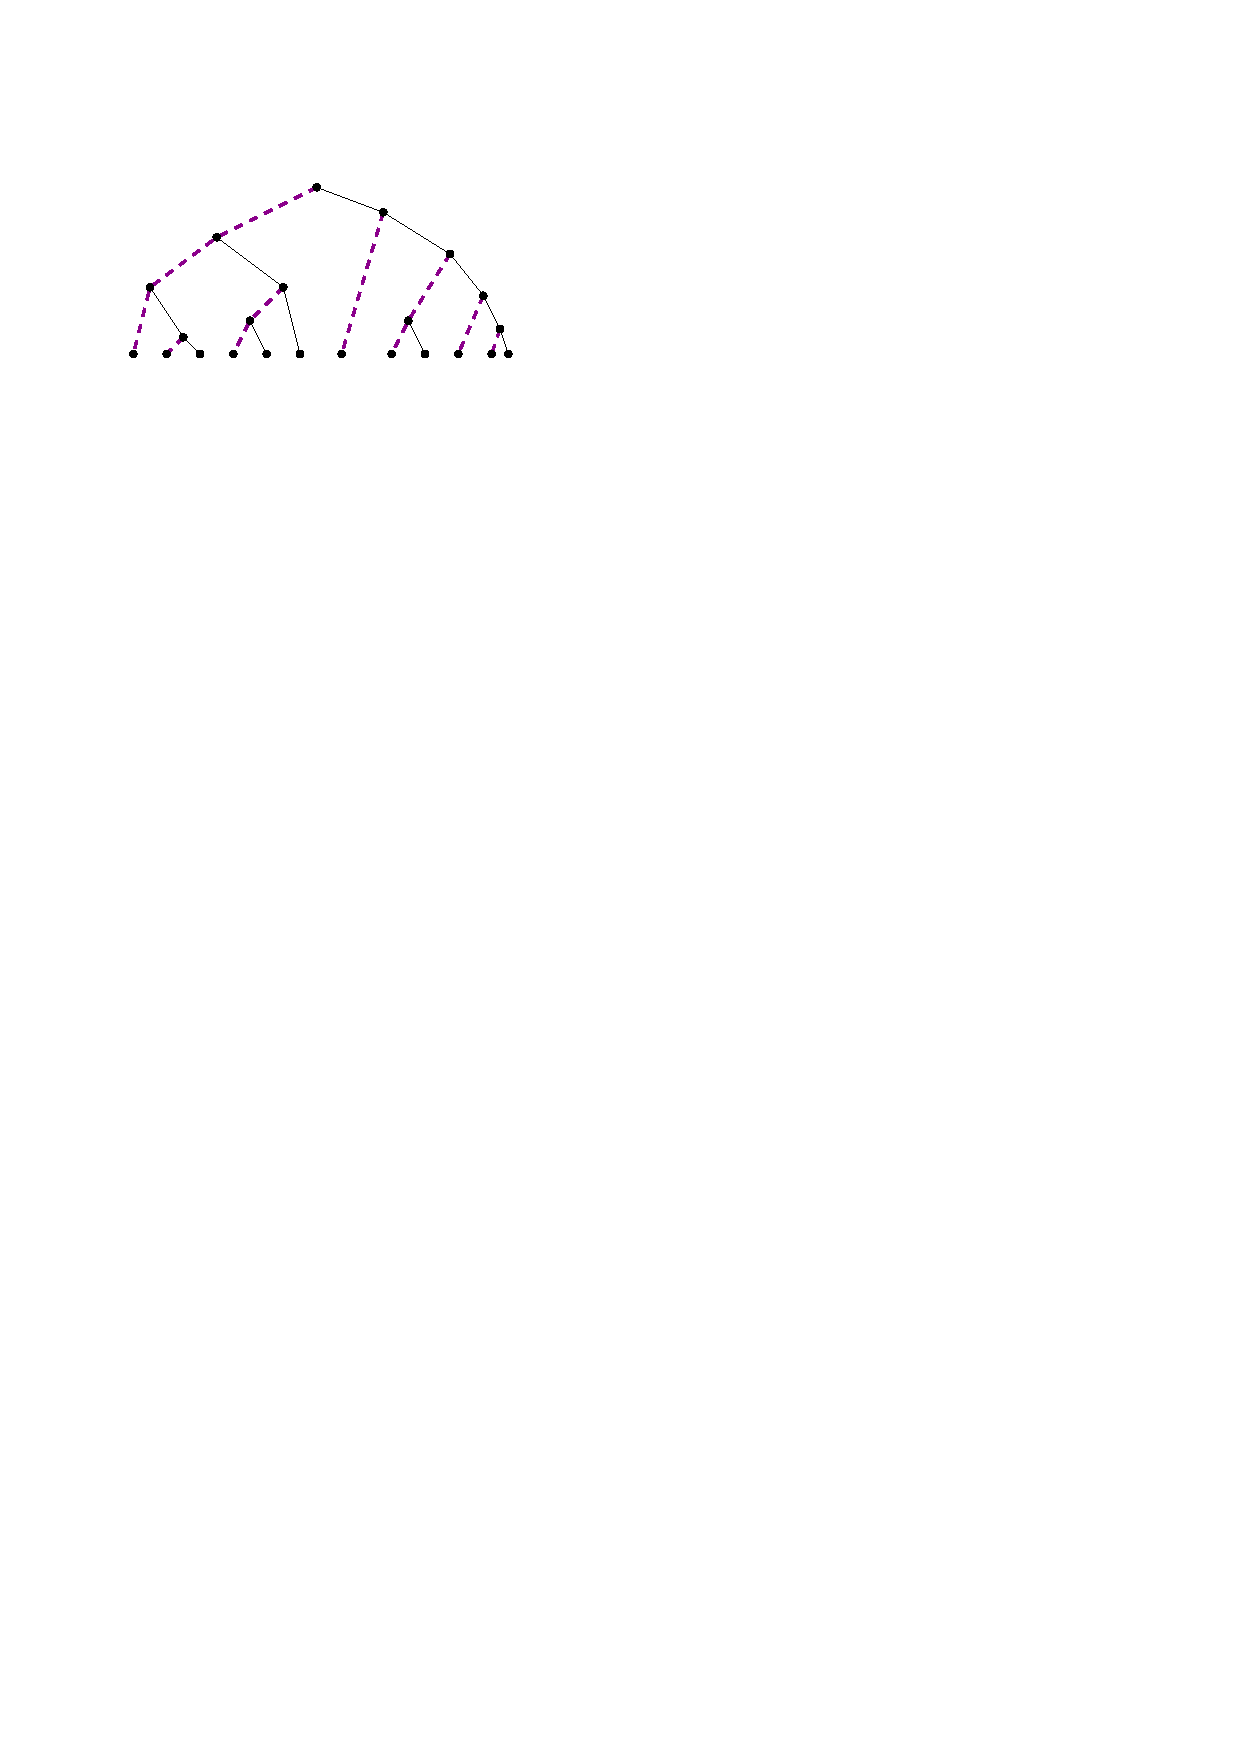
\includegraphics{pathdecomp}
\caption{For each leaf $v'$ of $T$, we connect the nodes
$v \in T$ by a dashed line for which $v$ is the leftmost leaf in $T_v$.
Considering these
subpaths for all leaves in $T$, we obtain a \emph{path decomposition}
of $T$ (shown in dashed).}
\label{fig:pathdecomp}
\end{figure}
To do this, we observe the following: let $v' \in T$ be 
a leaf in $T$. Then, $v'$ is the leftmost (or rightmost)
leaf in the subtrees of at most $w + 1$ ancestors $v$ of $v'$ (including $v$).
Furthermore, all these nodes form a subpath (more precisely,
a prefix) of the path from $v$ to the root, see Figure~\ref{fig:pathdecomp}.
Hence, if we store the nodes of 
this subpath in a balanced binary tree that supports a split
and a join operation,
we can obtain $O(\log w)$ update and query time
to find the leftmost (or rightmost) element in $T_v$
for each $v \in T$.
However, we need that the update and query time for this
data structure
depend on \emph{height} of the query node $v$, i.e., 
the number of edges on the path from
$v$ to the desired leaf.
Thus, we partition the possible heights
$\{0, 1, \dots, w\}$ of the nodes on a 
subpath into the sets
$T_{-1} = \{0\}$, $T_i =[2^i, 2^{i+1})$, for $i = 0,\dots,
\lfloor \log w  \rfloor$. 
The nodes in each set are stored in a balanced binary tree, and the 
roots of the trees are linked together, in order. 
The height of the $i$-th binary 
search tree is $\log |T_i| = O(i)$. Furthermore, if a query node
of height $h$ is given, 
it is contained in $T_{\lfloor \log h \rfloor}$, see 
Figure~\ref{fig:queryds}.
\begin{figure}
\centering
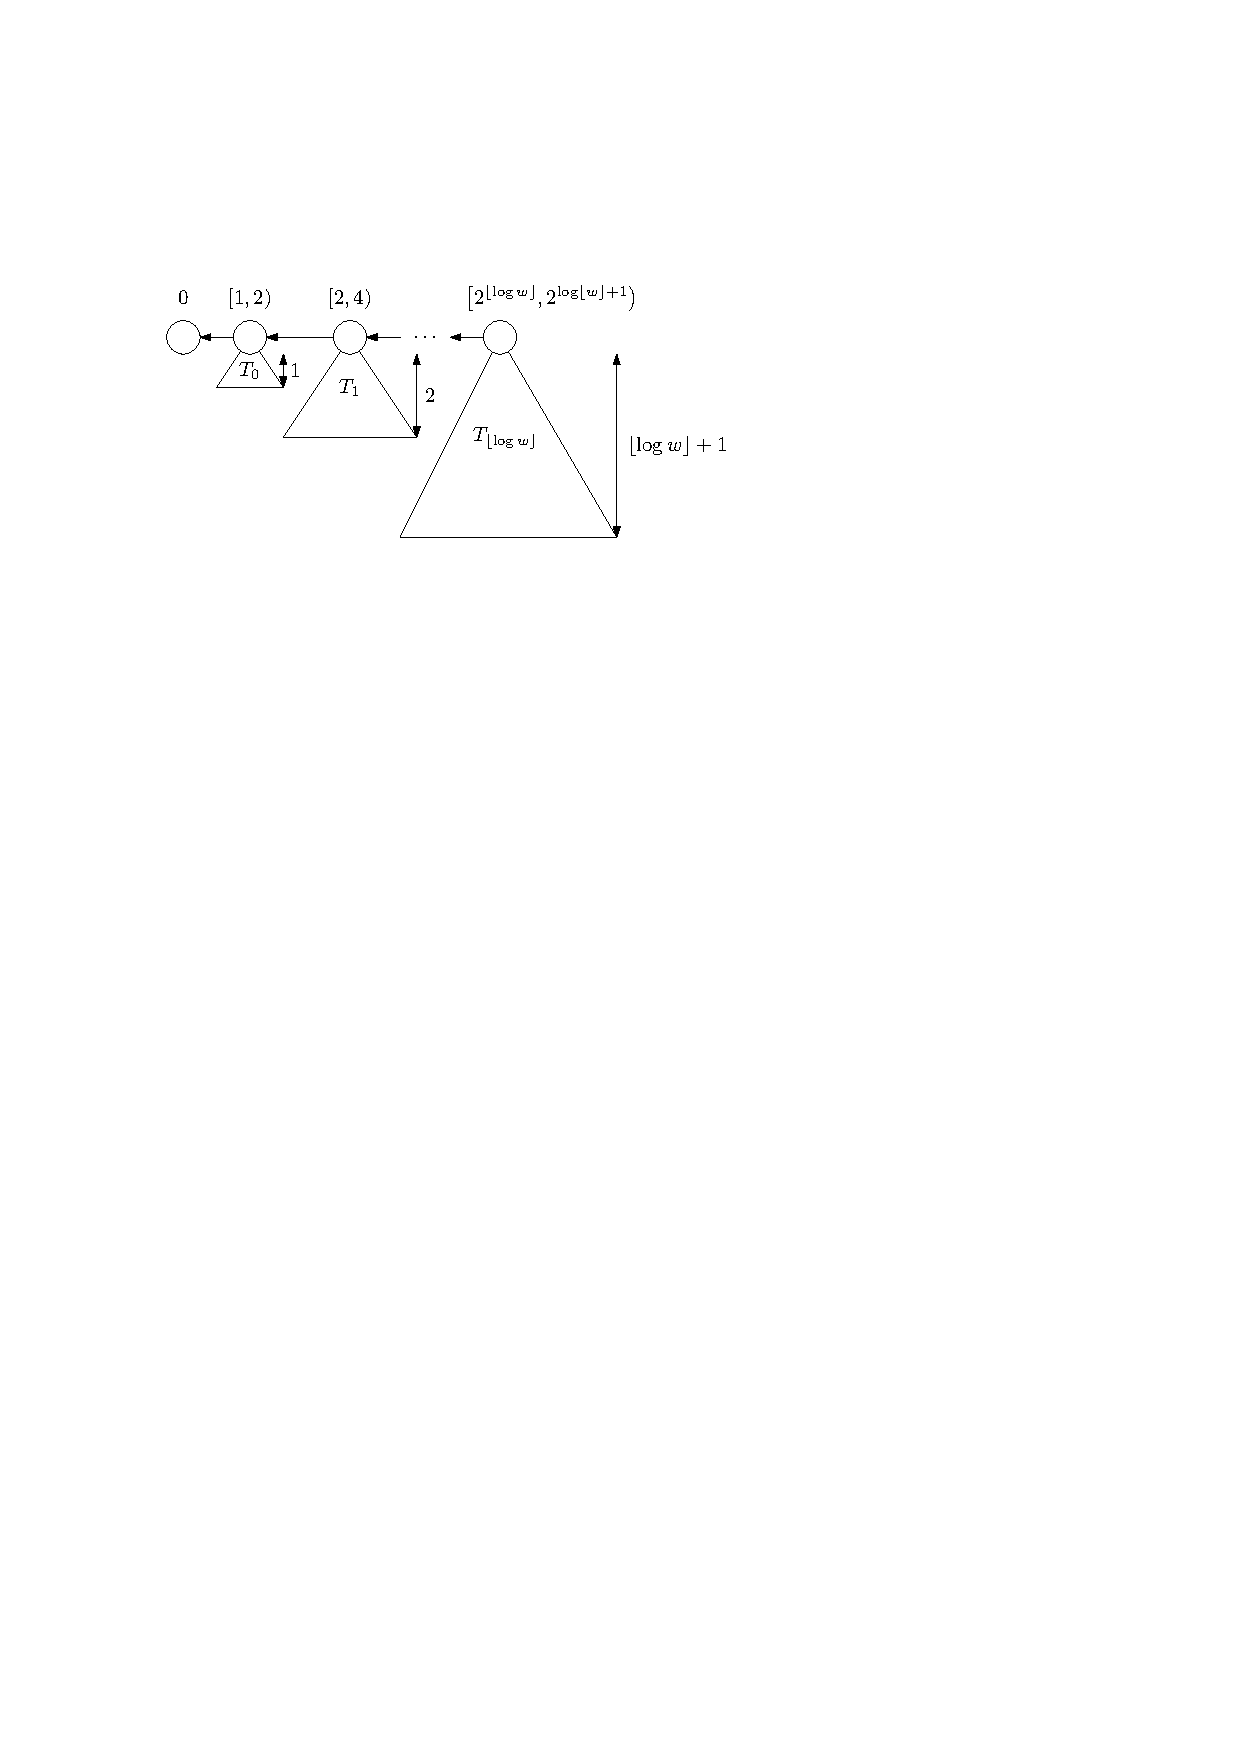
\includegraphics{queryds}
\caption{The data structure for a subpath. We group the nodes
in the subpath according to their heights, where the groups
grow exponentially in size. Each group is stored in a
balanced tree. The roots are joined in a linked
list. With this data structure, a node $v$ of height $h$ can
find the leftmost leaf in the subtree $T_v$ in time $O(\log h)$.}
\label{fig:queryds}
\end{figure}


Moreover, the node in $T_{-1}$ is a leaf 
in $T$ and therefore the minimum of the whole subpath. Thus, 
the minimum of a subpath can be found from a given node 
$v \in T_i$ in $O(i)$ time by following the
pointers to the root of $T_i$ and the pointers left to $T_{-1}$.
If a node $v$ has height $O(\log d(q, S))$, 
then $v$ is stored in
the tree $T_{\lfloor O(\log \log d(q, S)) \rfloor}$. Thus, it takes 
$O(\log \log \log d(q, S))$ time to find the leftmost
or rightmost leaf in $T_v$.

Our structure supports the following update operations:
(i) \textbf{split}: given a subpath $\pi$ and a node $v$ on $\pi$, split 
the representation of $\pi$ into two representations, one for the 
\emph{lower} subpath from the leaf up to the child of $v$, and
one for the \emph{upper} subpath starting from $v$; and (ii) 
\textbf{join}: given a
representation of an upper subpath starting at a node $v$ obtained 
from an operation of type (i), and a representation for 
a lower subpath up to a child of $v$, join the two representations
into the representation for a joint subpath.
We can implement
both \textbf{split} and \textbf{join} in
 $O(\log h)$ time, where $h$ is the height of 
the node $v$ where the operation occurs, using appropriate
split and join operations on the binary search trees that
appear in the structure. 
This decomposition of $T$ into dynamically changing suppaths
is similar to the \emph{preferred paths decomposition} of
Tango trees~\cite{DemaineHaIaPa07}.

\subsection{Putting it Together}

We know from the Lemma~\ref{lemma:delta_lca_loglog_delta}, that 
the exit node of a query element $q$ has expected 
height $O(\log d(q, S))$.

\begin{lemma}
\label{lemma:delta_insert}
Let $S \subseteq \{0, 1\}^w$, and let $r \in \{0, 1\}^w$ be
a fixed random shift. Let $T$ be
a trie for 
$S + r$.  Given a string $q \in \{0, 1\}^2$,
We can insert or delete $q$ in $T$
in $O(\log \log d(q, s))$ expected time, where the expectation is 
over the random choice of the shift $r$.
\end{lemma}

\begin{proof}
To insert $q$ into $T$, we need to split an edge $(u,v)$ of $T$ into
two edges $(u,b)$ and $(b,v)$. This creates
exactly two new nodes in $T$, an inner node and a leaf node. 
The node $u$ is exactly $\exit(q)$, and it has expected height 
$h = O(\log d(q, S))$, by Lemma~\ref{lemma:delta_lca_loglog_delta}. 
Thus, it will
take $O(\log\log d(q, S))$ expected time to find
the edge $(u,v)$, by
Lemma~\ref{lem:delta_fast_expected_lca}.

Once the edge $(u,v)$ is found, the dictionary that stores
the z-fast trie
can be updated in constant time.
Now let us consider the update time of the 
dictionaries that store the sets $P$ and $Q$ of prefixes.
We may need to insert two new prefixes into $Q$, one
for the edge $(b, v)$ and one for the edge $(b,q)$. 
We also need  to
update the values for all the prefixes in $P$ that lie
on the edge $(b,v)$.
Finally, we may need to add a new the new prefixes
into $P$ that lie on the edge $(b,q)$.
This needs
$O(\log\log\log d(q,S))$ insertions and updates in expectation: we
have to insert or change the prefixes for all 
$i \geq 1$ with $w - 2^{2^i} \geq w - h$, where
$h$ is the expected height of $b$. By Lemma~\ref{lemma:delta_lca_loglog_delta},
the expectation of $h$ is $\Theta(\log d(q, S))$,
so the expectation of $i$ is $O(\log\log\log d(q, S)$.

After that, the leftmost and rightmost elements for the subtrees
of $T$ have to be updated. For this, we need to add one
subpath for the new leaf $q$, and we may need to split
a subpath at a node of height $O(\log d(q, S))$ and join
the resulting upper path with the newly created subpath. As we
have seen, this takes $O(\log \log d(q, S))$ time.

The operations for deleting an element $q$ from $S$ are symmetric.
\end{proof}

The following theorem summarizes our result.

\begin{theorem}
Let $r \in \{0, 1\}^w$ be picked uniformly at random.
After performing a shift of $\{0, 1\}^w$ by $r$, 
there is a data structure for the
dynamic predecessor problem such that 
query and update operations take $O(\log \log d(q, S))$ 
expected
time, where $q$ is the
requested element and 
$S$ is the current set in the data structure. At any point in time, 
the data structure needs $O(nw)$ bits of space, where $n = |S|$.
\end{theorem}


\subsection{Applications}

Bose~\etal~\cite{BoseDoDuHoMo13} describe how to combine their structure
with a technique of Chan~\cite{Chan02} and random 
shifting~\cite[Chapter~11]{HarPeled11} for obtaining a data structure for 
distance-sensitive
approximate nearest neighbor queries on a grid.
More precisely, let $d \in \N$ be the fixed dimension, 
$U = \{0, \dots, 2^{w}-1\}$ be the universe, and
let $\eps > 0$ be given.
The goal is to maintain a dynamic set $S \subseteq U^d$ under
insertions, deletions, and \emph{$\eps$-approximate
nearest neighbor queries}: given a query point $q \in U^d$,
find a $p \in S$ with $d_2(p,q) \leq (1+\eps)d_2(p, S)$.
Plugging our predecessor structure into the structure of
Bose~\etal~\cite[Theorem~9]{BoseDoDuHoMo13}, we can
immediately improve the space requirement of their structure to linear:
\begin{theorem}
Let $U = \{0, \dots, 2^w-1\}$ and let $d$ be a constant.
Furthermore, let $\eps > 0$ be given.
There exists a data structure that supports $(1+\eps)$-approximate
nearest neighbor queries over a subset $S \subseteq U^d$ in 
$(1/\eps^d)\log\log d_2(p, S))$ expected time and insertions and deletions
of elements of $U^d$ in $O(\log\log d_2(p, S))$ expected time.
Here, we use the Euclidean distance between the query element $p$
and $S$. At any point in time, the data structure requires $O(n)$
words of space, where $n  = |S|$.
\end{theorem}

As a second application, Bose~\etal~\cite{BoseDoDuHoMo13}
present a data structure for dominance queries on a grid,
based on a technique of Overmars~\cite{Overmars88}.
Again, let $U = \{0, \dots, 2^w-1\}$, and let $S \subseteq U^2$,
$|S| = n$ be given. The goal is to construct a data structure
for \emph{dominance queries} in $S$. That is, given a query point
$q \in U^2$, find all points $p$ in $S$ that \emph{dominate} $q$,
i.e., for which we have $p_x \geq q_x$ and $p_y \geq q_y$, there
$p_x$, $p_y$ and $q_x$, $q_y$ are the $x$- and $y$-coordinates 
of $p$ and $q$.

Again, using our structure, we can immediately improve the
space requirement for the result of 
Bose~\etal~\cite[Theorem~10, Corollary~13]{BoseDoDuHoMo13}.

\begin{theorem}
Let $U = \{0, \dots, 2^w-1\}$, and let $S \subseteq U^2$, $|S|=n$
be given. There exists a data structure that reports the points in $S$
that dominate a given query point $q = (a,b) \in U^2$ in expected time
$O(\log\log(h+v) + k)$, where $h = 2^w - a$, $v = 2^2-b$, and $k$
is the number of points in $S$ dominated by $q$.
The data structure uses $O(n \log n)$ space.
\end{theorem}


\section{Globally sensitive predecessor search}

We can apply Theorem~\ref{thm:pred-long} to improve 
exponentially over the bound by Demaine, Jones, and 
\Patrascu~\cite{DemaineJoPa04}, which gives an algorithm whose running time
depends on the largest and smallest distance between the elements of $S$. 
More precisely, let
$\Delta_M$ and $\Delta_m$ be, respectively, the largest and smallest distance
between two consecutive elements of $S$.
\begin{corollary}
\label{cor:deltadelta}
Using an index of $O(n\log w)$ bits, it is possible to answer predecessor
queries in time $O(\log\log(\Delta_M/\Delta_m))$.
\end{corollary}
\begin{proof}
We use a standard ``universe reduction'' argument, splitting 
the universe $\{0, 1\}^w$ by grouping strings that have the same 
most significant $\lceil \log
n\rceil$ bits. Each subuniverse $U_i$ has size 
$2^{w-\lceil \log n\rceil}=O(2^w/n)$, and we let $S_i=S\cap U_i$. 
Using a constant-time
prefix-sum data structure \wolfgang{Reference?}, 
we keep track of the rank in $S$ of the smallest
element of $S_i$, and we build the indices that are necessary for
Algorithm~\ref{algo:pred-long} for each $S_i$ 
(seen as a set of strings of
length $w-\lceil \log
n\rceil$). 
Thus, we can answer a query $q$ in time 
$O(\log(w-\lceil \log n\rceil -\log D(q, S_i))$, where 
$U_i$ is the subuniverse containing $q$. Now,
note that $\Delta_M \geq 2^w/n$, and that 
\[
\Delta_m \leq q^+ - q^- = (q^+ - q) + (q - q^-)
\leq 2D(q, S) \leq 2D(q, S_i),
\]
(unless $q$ is the smallest or the
largest element of $S_i$, but this case can be dealt with in constant time). 
The bound follows immediately.
\end{proof}

\section{Finger predecessor search}

We conclude with a generalisation of long-distance search 
that builds on previous results~\cite{BelazzouguiBoPaVi11b}.
Using $O(n w^{1/c})$ bits of space (for any positve integer $c$), 
it is possible to answer \emph{weak prefix search} queries in 
constant time. A weak prefix search query takes a prefix 
$p \in \{0, 1\}^*$, and it returns the minimum and maximum
index of an element in $S$ that has prefix $p$; if no such element exists,
the results are arbitrary (hence the ``weak'' qualifier), but 
a single access to the set $S$ is sufficient
to rule out this case and to always get a correct result. Thus, we will be
able to compute $\lrange(\cdot)$, $\rrange(\cdot)$ and $\extent(\cdot)$ 
on arbitrary elements of $\Pref(S)$ in constant time. 
As a consequence, $\pred(q,t)$ can also
be extended to return a correct value for every $t$ with 
$q[0, t - 1] \in \Pref(S)$.

The basic idea of Algorithm~\ref{algo:finger} is to use 
a \emph{finger} $y \in S$ to locate quickly an extent $e$ 
that is a prefix of $q$ and that has the property 
that $w - |e| \leq \log |q - y|$. The extent
is then used to accelerate an algorithm essentially identical
Algorithm~\ref{algo:pred-long}, but applied to a reduced universe 
(the strings starting with $e$); the running time thus becomes
$O(\log(w - |e| - \log D(q, S)|) = O(\log(\log|q - y|- \log D(x, S)))$.

\begin{algorithm}
\KwIn{a nonempty string $q \in \{0, 1\}^w$ and a $y \in S$ such that $y < q$}
\KwOut{an index $i$ with $S[i] = q^-$}

$t \gets \max\{\,s \mid y[0, s - 1] + 1 \preceq q\,\}$\;
$e \gets \extent(y[0, t - 1] + 1)$\;
\If{$y[0, t - 1] + 1 \not\preceq e$}{%
  \Return $\rrange(y[0, t - 1])$
  \label{line:finger_ret1}
}
\tcp{$y[0, t - 1] + 1\not\in\Pref(S)$} 
\If{$e \not\prec q$}{% 
  \Return{$\pred(q, t)$
\label{line:finger_ret2}
  }
}
\tcp{$q$ exits between $y[0, t - 1] + 1$ and $e$} 
$a \gets 0$\;
\tcp{Now $e \prec q$ and $w - |e| \leq \log |q - y|$} 
\While{$a < (w - |e|)/2$}{%
  $m \gets \text{least power of~2 in $\{a - |e|+ 1, \dots, w - |e| -1\}$}$\;
  $p \gets q[0, m + |e| - 1]$\;
  \If{$p\not\in\Pref(S)$}{%
    \Return $\fbs^-(q, a + |e|, m +|e|)$
  }
  \If{$S[\lrange(p)]\geq q$}{%
    \Return{$\lrange(p)-1$}
  }
  \If{$S[\rrange(p)] < q$}{%
    \Return{$\rrange(p)$}
  }
  $a \gets |\extent(p)|-|e|$ 
  \tcp{This is a valid extent}
}
\Return{$\fbs^-(q, a +|e|,w)$}
\caption{Long-distance finger-search speedup.}
\label{algo:finger}
\end{algorithm}


\begin{theorem}
\label{th:finger}
Algorithm~\ref{algo:finger} returns the predecessor 
of a query string $q$ given
a finger $y\in S$, with $y < q$, in time 
$O(\log(\log|q - y|-\log D(q,S)))$, using an 
index of $O(n w^{1/c})$ bits 
of space, for any $c$ 
(in addition to the space needed to store the elements of $S$).
\end{theorem}

\begin{proof}
First, we show that the algorithm is correct. 
If we exit at the first return instruction
in line~\ref{line:finger_ret1},
$y[0, t - 1] + 1$ is not in $\Pref(S)$, 
which implies that $q^-$ is prefixed by $y[0, t - 1]$, 
and thus the output is correct. If we exit at 
the second return instruction in 
line~\ref{line:finger_ret2}, $q$
exits at the same node as $y[0, t - 1] + 1 = q[0, t - 1]$. 
Otherwise, $e$ is an extent
that is a proper prefix of $q$, and the remaining part 
of the algorithm is exactly Algorithm~\ref{algo:pred-long} 
applied to the set of strings of $S$ that are prefixed by $e$, 
with $e$ removed (the algorithm is slightly simplified 
by the fact that we can test membership to $\Pref(S)$ and compute
extents for every prefix). Correctness is thus immediate.

All operations are constant time, except for the last loop. 
Note that as soon as $m + |e| \geq  w - \log D(q, S)$, 
the loop ends or a prefix of $q$ is found (as in the
proof of Algorithm~\ref{algo:pred-long}), 
and this requires no more than $\log(w - |e| - \log D(q, S))$ 
iterations; moreover, $m \leq 2a$ (because there is always
a power of $2$ in the interval 
$[a + 1, 2a]$), so the fat binary search in the first
return will take no more than
\[
\log(m - a) \leq \log a \leq \log (w - |e| - \log D(q, S))
\]
steps.
If the loop exits naturally, then there is a 
prefix $e'$ of $q$ belonging to $\Pref(S)$ 
and longer than $(w + |e|)/2$, hence by
Lemma~\ref{lemma:shortinprefs}, 
we have $w - \log D(q, S) \geq (w + |e|)/2$; 
the fat binary search at the
end takes time 
\[
O(\log (w -(a + |e|))) = O(\log (w - |e'|))
=O(\log( w/2 - |e|/2))) =O(\log(w-|e|-\log D(q,S))),
\]
within the prescribed time bounds.
\end{proof}

\section{An Improvement through Higher Degrees}

\subsection{Faster Fat Binary Search}

We now show how to slightly improve our running times.
The idea is to interpret the elements in $S$ as
words over the larger alphabet $\{0, 1\}^{\lceil \log w / 2 \rceil}$.
This increases the degree of the trie $T$, but the additional
work due to the higher degree will be only constant, because it can
be handled through constant-time word operations.

More precisely, we increase the degree of our trie $T$ 
to $\sqrt{w}$. For each node 
$v$, we store the symbols from $\{0, 1\}^{\lceil \log w / 2 \rceil}$
that correspond to the children of $v$
in a children predecessor data 
structure $D_v$. 
The children predecessor data structure 
$D_v$ is just an array of the symbols, in sorted order. 
The array needs just $O(\log w)$ bits for each symbol
Thus the children predecessor structure $D_v$ fits in at most 
$\sqrt{w} \cdot {\log w}$ bits, and a predecessor search can 
be done in constant time, using appropriate word-RAM operations
\wolfgang{Explain how? What exactly do we do?}. 
The total space needed for the $D_v$ structures, over all $v \in T$,
is $O(n\log w)$ bits. 

By grouping
$w/\lceil\log w/2\rceil$ consecutive 
bits as a character, we interpret the 
elements of $S$ as strings of length $w/\lceil\log w/2\rceil$ 
over the alphabet $\{0, 1\}^{\lceil \log w / 2 \rceil}$ (using
appropriate padding).
The notions of name, 
extent, and handle of a node in $T$ remains unchanged, except for 
the difference that they are now strings over 
$\{0, 1\}^{\lceil\log w/2\rceil}$ instead of $\{0,1\}$. 
The implementation of the function $Z$ is also the same as before. 
In addition to function $Z$, we store for each node a children
predecessor structure. Since this needs $O(\log w)$ bits for each
child node, this adds 
$O(n\log w)$ bits to the total space. 
The definition of an exit node for a string $q \in \{0, 1\}^*$ 
is also slightly changed. 
It is now as follows:
\begin{enumerate}
\item the only node $v$ such that $n_v$ is a prefix of $q$ and 
either $e_v = q$ or $e_v$ is not a prefix of $q$, 
if such a node exists (in this case, we call it 
and exit node of type $1$). 
\item if no such node exists, then the exit node 
is defined as the only node $v$ such that $e_v$ is prefix of 
$q$ and for any child $w$ of $v$, we have that $n_w$ is not a prefix of 
$q$ (in this case, $v$ is called an exit node of type $2$). 
\end{enumerate}

Now the fat-binary search is also unchanged except that the returned exit node has a slightly different definition. In order to finish a predecessor search we need a final step. We first determine whether the type of the exit node $\alpha=\exit x$ as follows: we use the range locator to determine the extent of $\alpha$. If $e_\alpha$ is prefix of $x$ but $e_\alpha\neq x$ then we conclude that we have a type $1$ exit node. Otherwise, we conclude that we have a type $2$ exit node. 
If the $\alpha$ was an exit node of type $1$, then the predecessor search is finished exactly as before. On the other hand if the exit node is of type $2$ then we finish the search as follows: we use extract character $c=x[|e_\alpha|+1]$ and do a predecessor search for $c$ on $D_\alpha$. This predecessor search returns the label of a node $\beta$ which is child of $\alpha$. The name of $\beta$ will be obtained by concatenating $e_\alpha$ with the label of $\beta$. Finally the predecessor of $x$ will be the last element in the range under $\beta$ which can obtained by calling the range locator for $n_\beta$. 
Once we have recognized the type of the exit node, we can conclude the predecessor search as follows:

\subsection{Faster Short Distance sensitive predecessor search}

We now do short distance sensitive predecessor search in time $O(\log\frac{\log d(x,S)}{\log w})$. Once we get to level $\log\log d(x,S)-\log\log w$, we do fat binary search. The fat-binary search stops after $\log\log d(x,S)-\log\log w$ steps and the final search is done as describes in the previous section. Of course the definition of $P$ and $Q$ are changed to reflect the fact that now all the keys are viewed as strings over alphabet $[2^{\lceil\log w/2\rceil}]$. Thus $P$ is redefined as follows:

\[
	P=\bigl\{\,x\bigl[0..\frac{w}{\lceil\log w/2\rceil}]-2^{2^i}\bigr) \mid x \in  S \text{ and }
	i=0,1,\dots,\lfloor\log(\log \frac{w}{\lceil\log w/2\rceil} - 1)\rfloor\,\bigr\}.
\]
And $Q$ keeps exactly the same definition. 
\[
Q=\bigcup_{\text{node $\alpha$}}\min{}_\preceq\{\,p\in P\mid n_\alpha\preceq p\preceq e_\alpha\,\}
\]
Now the algorithm for short distance sensitive search is exactly as before except that the searched key $x$ is now considered as a key over alphabet $[2^{\lceil\log w/2\rceil}]$ and that the number of iteration of the while loop is upper bounded by $\frac{w}{2\lceil\log w/2\rceil}$ instead of $w/2$
\begin{theorem}
\label{thm:pred-short}
We can build an index that returns the predecessor of $x$
in time $O(\log\frac{\log d(x,S)}{\log w})$, and requires $O(n \log w )$
bits of space (in addition to the space needed to store the elements of $S$).
\end{theorem}


%To see why the search now takes $O(\log\frac{\log d(x,S)}{\log w})$. The reason is that whenever $d(x,S)\leq $
\subsection{Faster and smaller long sensitive search}
We show how to achieve $O(\log\frac{w-\log D(x,S)}{\log w})$ query time with space $O(n\log\log w)$ bits. 
We first cut the table into blocks of size $b=\log w$ keys. Then we build a new table that contains the first key of each block which thus contains $n/\log w$ keys in total. We let $S'$ denote that set of elements. It is easy to see that $D(x,S')\geq D(x,S)$ for any $x$. 
We build a distance sensitive index on this new table. This index will occupy space $O(n)$ bits in total. We now show how to index each block using $\log\log w$ bits per key. We will build a local index on each block but only on the $\log^2 w$ most significant bits of the keys in each block. We divide each block into $\sqrt{\log w}$ sub-blocks each containing $\sqrt{\log w}$ keys forming a tree with two levels and nodes having fan-out $\sqrt{\log w}$. The upper level will have one node that indexes all the first keys in the sub-blocks. For each node, we build an index consisting in a compacted trie on the $\log^2 w$ MSBs of the keys in the node. Such an index will use $2(\log\ell+1)$ bits per key where $\ell$ is the length of the keys. It was described by Grossi et al~\cite{GRR09} and is called an SB-node and is based on the string B-tree approach~\cite{FG99}. The main property of the local index is that after probing the index, we can answer to a predecessor query by only reading one single key . In our case, we will index only the $\log^2 w$ MSBs of the keys stored in each node and thus use $2\log\log w$ bits per key. In order to answers queries for each node, we will use a precomputed table that will give us the position to be probed in the table in constant time, based on the node encoding. The precomputed table stores all the answers for all the queries for all possible SB-nodes. Note that the node stores $\sqrt{\log w}$ elements and is encoded using a patricia trie that occupies $2(\log\ell+1)=O(\log(\log^2w))=O(\log\log w)$ bits per element. The precomputed table will thus use $2^{O(\sqrt{\log w}\cdot \log\log w)}\cdot\log^2w\cdot\frac{1}{2}\log\log w=o(w)$ bits of space to store the answers to all possible queries (that is to give) on a node. That is the total number of possible nodes is  $2^{O(\sqrt{\log w}\cdot \log\log w)}$, a query is description needs $\log^2w$ bits,  and the answer to query is a position among $\sqrt{\log w}$ keys which needs $\frac{1}{2}\log\log w$ bits to be described.

\paragraph{Long-distance sensitive queries}
A long-distance sensitive query will be done exactly (algorithm 3) as before except that now that the searched key $x$ is now considered as a key over alphabet $[2^{\lceil\log w/2\rceil}]$. As before we start searching for prefixes of $x$ of lengths $2^{2^i}$ for $i=1,2,\ldots$ (which translates to lengths $2^{2^i}\log w$ bits) in order to find the longest prefix of length of the form $2^{2^i}$ and then complete by a call fat-binary search to find the predecessor among the sampled keys (recall that we are sampling only one every $\log w$ keys) and we will have isolated one block of size $b=\log w$ that contains the predecessor of $x$. To complete the search for the predecessor among all the keys of $S$, we do the following: if the search stopped and called the fat-binary search at step $i$, we first check whether $i\leq\log\log w$:
\begin{enumerate}
\item If this is not the case (that is $i>\log\log w$), We complete the search with a binary search on the block of the predecessor that contains $\log w$ elements in $O(\log\log w)$ time. Note that the fact that $D(x,S)\geq 2^{w-\log^2w}$ automatically means that $D(x,S')\geq 2^{w-\log^2w}$ which in turn implies that the search finishes before step $\log\log w$. Thus the search finishing after step $\log\log w$ implies that $D(x,S)< 2^{w-\log^2w}$ and thus that $\log\log w\leq \log\frac{w-\log D(x,S)}{\log w}$
\item If this was the case (that is $i\leq\log\log w$), then we do a local predecessor search on $x'$ (where $x'$ is formed with the $\log^2 w$ MSBs of $x$) on the keys of the block using the local index. If we find a single key $y$ whose $\log^2 w$ MSBs are equal $x'$, then we are done as we only need to compare $x$ and $y$. If we have found a range of more than one whose key $\log^2 w$ MSBs are equal  to $x'$, then we check that $x$ is in between the largest and the smallest keys of the range that share $x'$ (keys that have $x'$ as their $\log^2w$ MSBs). Then we have two cases
\begin{enumerate}
\item If we find that it is not the case (that is that $x$ is smaller or larger than all the keys that have $x'$ as their $\log^2w$ MSBs), then we can have effectively found the predecessor of $x$ which will be either the largest keys that have $x'$ as its $\log^2w$ MSBs or the predecessor of the first key $x'$ as its $\log^2w$ MSBs. 
\item If this was the case then we know for sure that $\log D(x,S)\leq w-\log^2 w$ and just do binary search on the whole block in time $O(\log\log w)$  which is within our target query time as we have $\log\frac{w-\log D(x,S)}{\log w}\geq \log\frac{w-(w-\log^2w)}{\log w}=\log\log w$. 
\end{enumerate}
\end{enumerate}
It is trivial to transform a long-distance sensitive result into a globally sensitive result and get the following theorem. 
\begin{theorem}
\label{thm:pred-long2}
We can build an index that returns the predecessor of $x$
in time $O(\log\frac{w-\log n-\log D(x,S)}{\log w})$, and requires $O(n \log\log w )$
bits of space (in addition to the space needed to store the elements of $S$).
\end{theorem}

\subsection{Faster Finger Search}
The finger search result can easily be deduced 
from the log-distance predecessor result. The details are omitted. 
\begin{theorem}
\label{th:finger_faster}
We can build an index that returns the predecessor 
of an input string $q \in \{0, 1\}^2$ given
a finger $y \in S$, with $y < q$, 
in time $O(\log\frac{\log|q - y|-\log D(q, S)}{\log w})$, using  
$O(n w^{1/c})$ bits 
of space, for any $c$ 
(in addition to the space needed to store the elements of $S$).
\end{theorem}



\bigskip
\noindent\textbf{Acknowledgments.}
We thank the anonymous reviewers for numerous
insightful comments that improved the quality of the paper.
\wolfgang{TODO}

\hyphenation{ Vi-gna Sa-ba-di-ni Kath-ryn Ker-n-i-ghan Krom-mes Lar-ra-bee
  Pat-rick Port-able Post-Script Pren-tice Rich-ard Richt-er Ro-bert Sha-mos
  Spring-er The-o-dore Uz-ga-lis }


\bibliographystyle{abbrv}
\bibliography{journal}

\end{document}
